% Working atlas figure snippets; paths relative to repository root.
% Figures are source-bound and individually QC reviewed.

\begin{figure}[tbp]
  \centering
  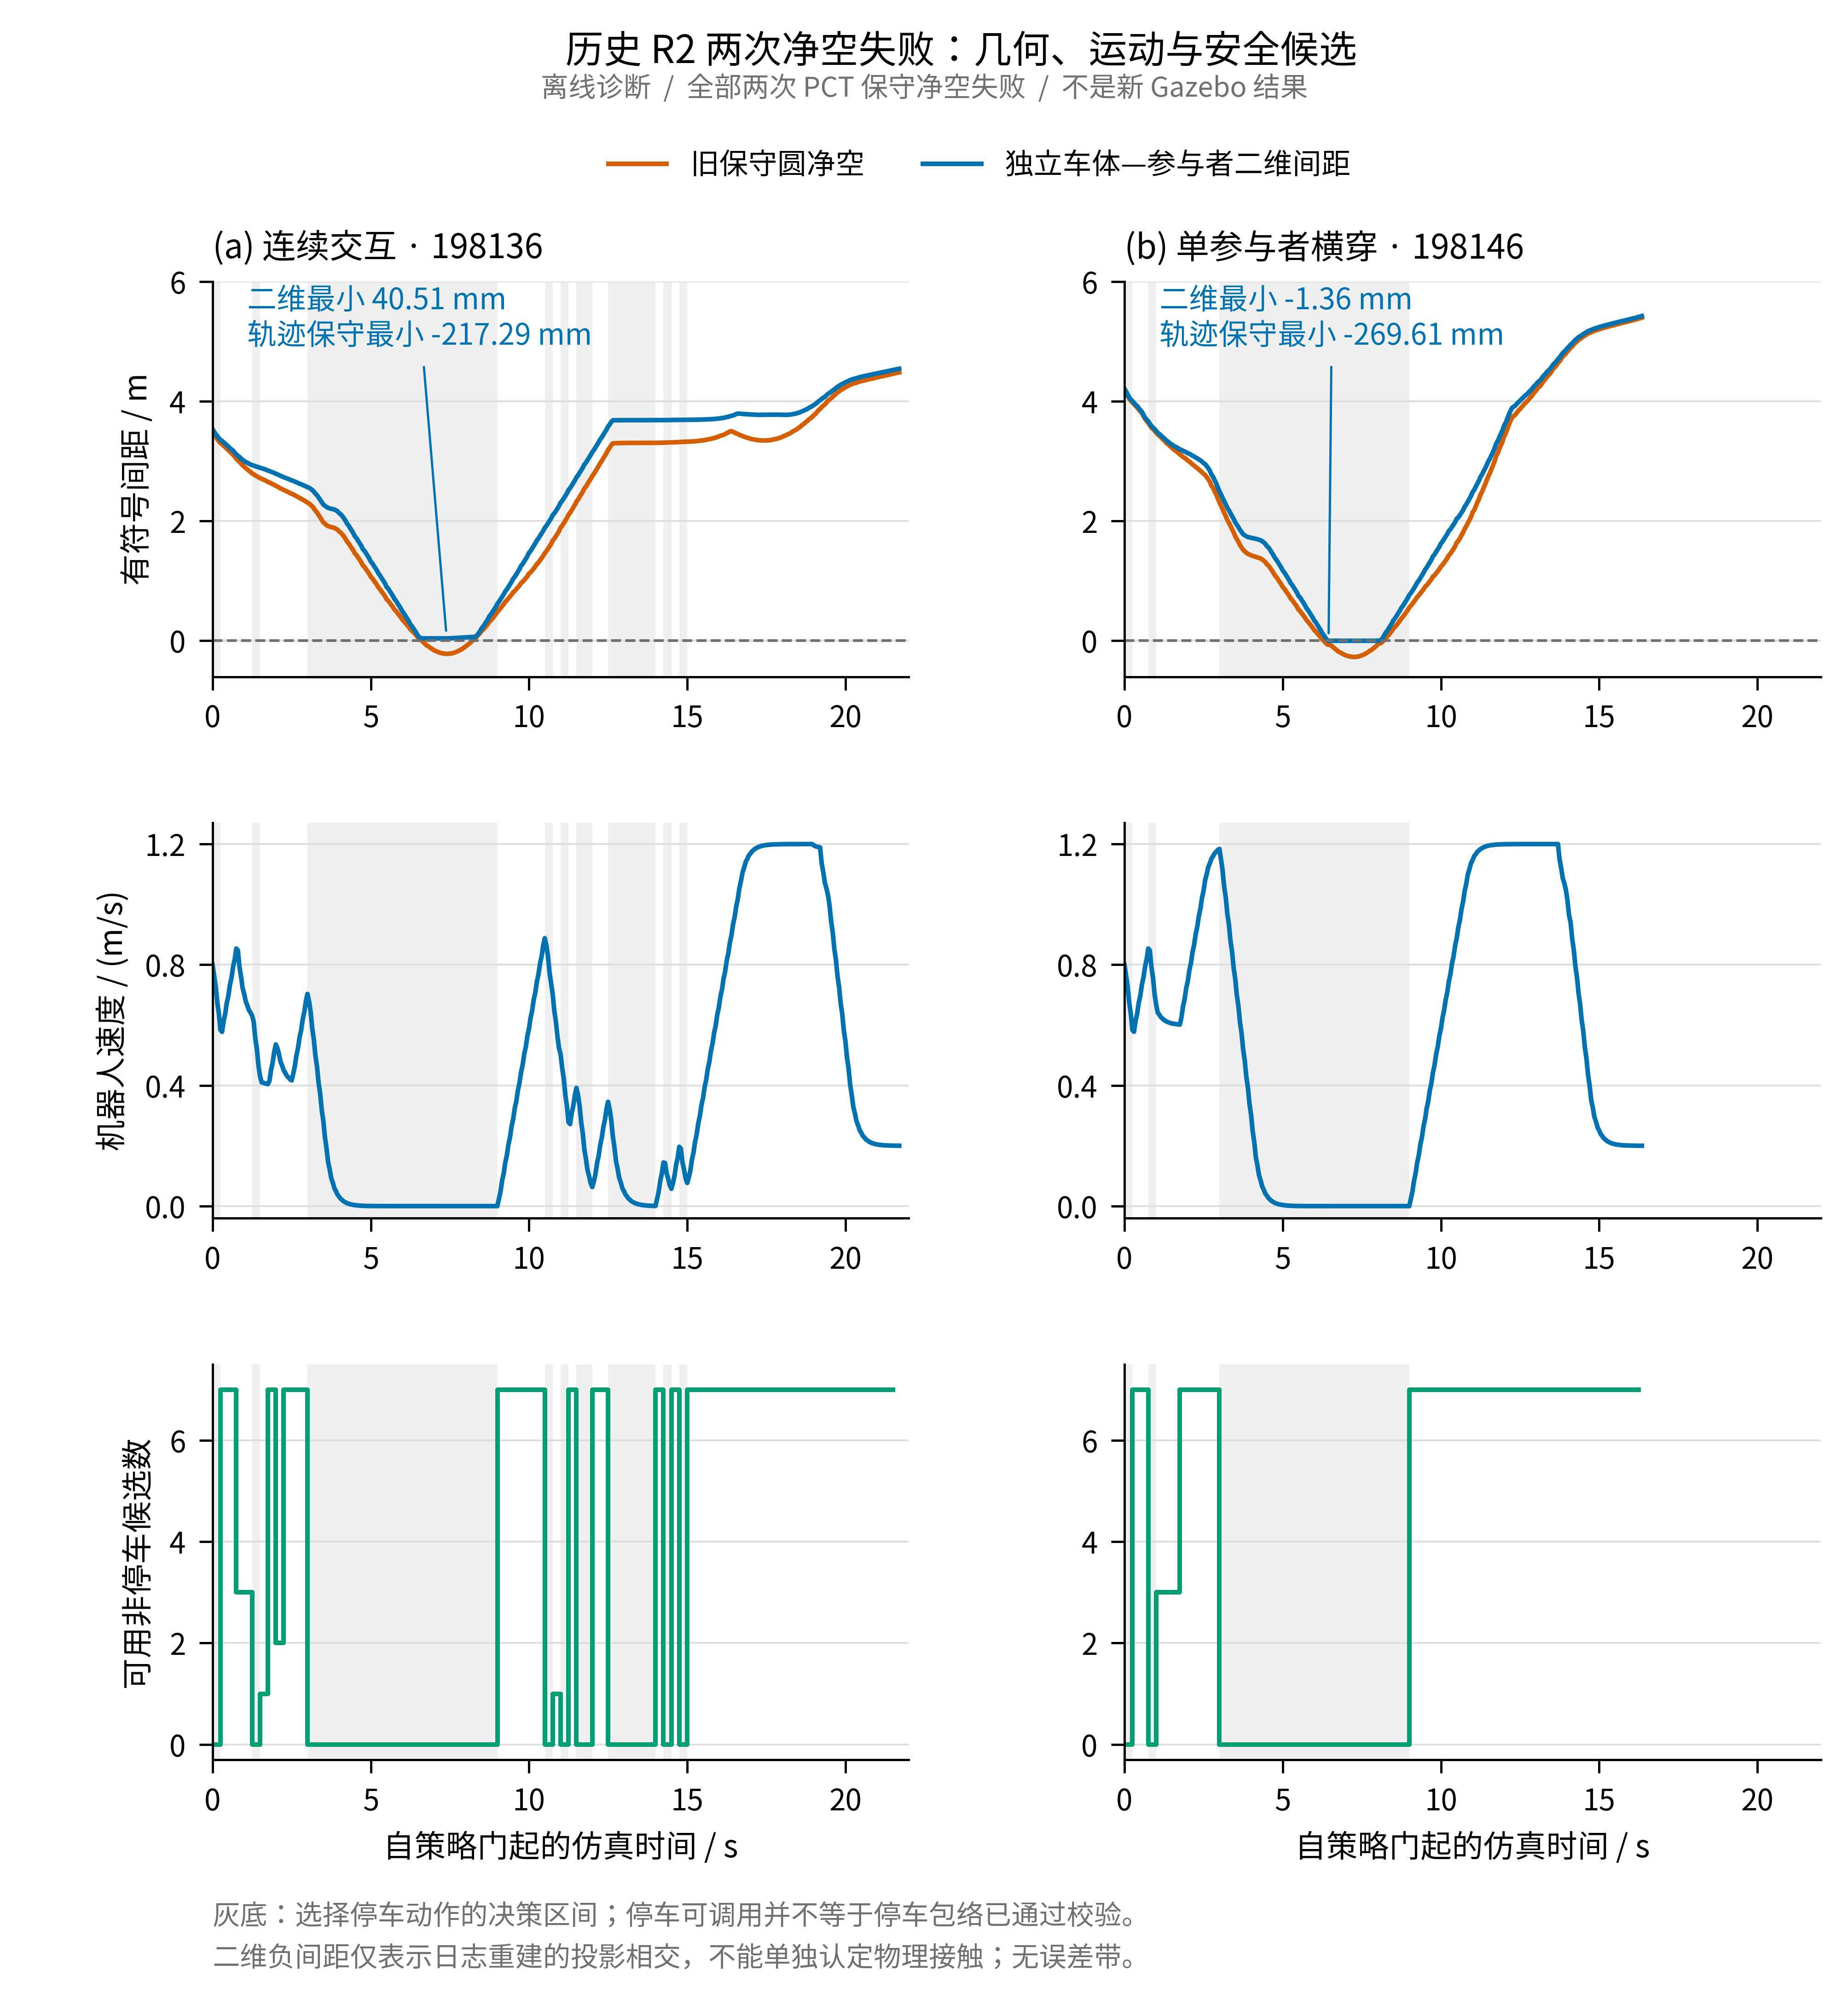
\includegraphics[width=\linewidth]{artifacts/astra_gazebo_20260926/visuals/plots/historical_diagnosis/r03/H01.png}
  \caption{历史 R2 两次冲突失败。历史误选发生在何种几何和运动关系下}
  \label{fig:astra-h01}
\end{figure}

\begin{figure}[tbp]
  \centering
  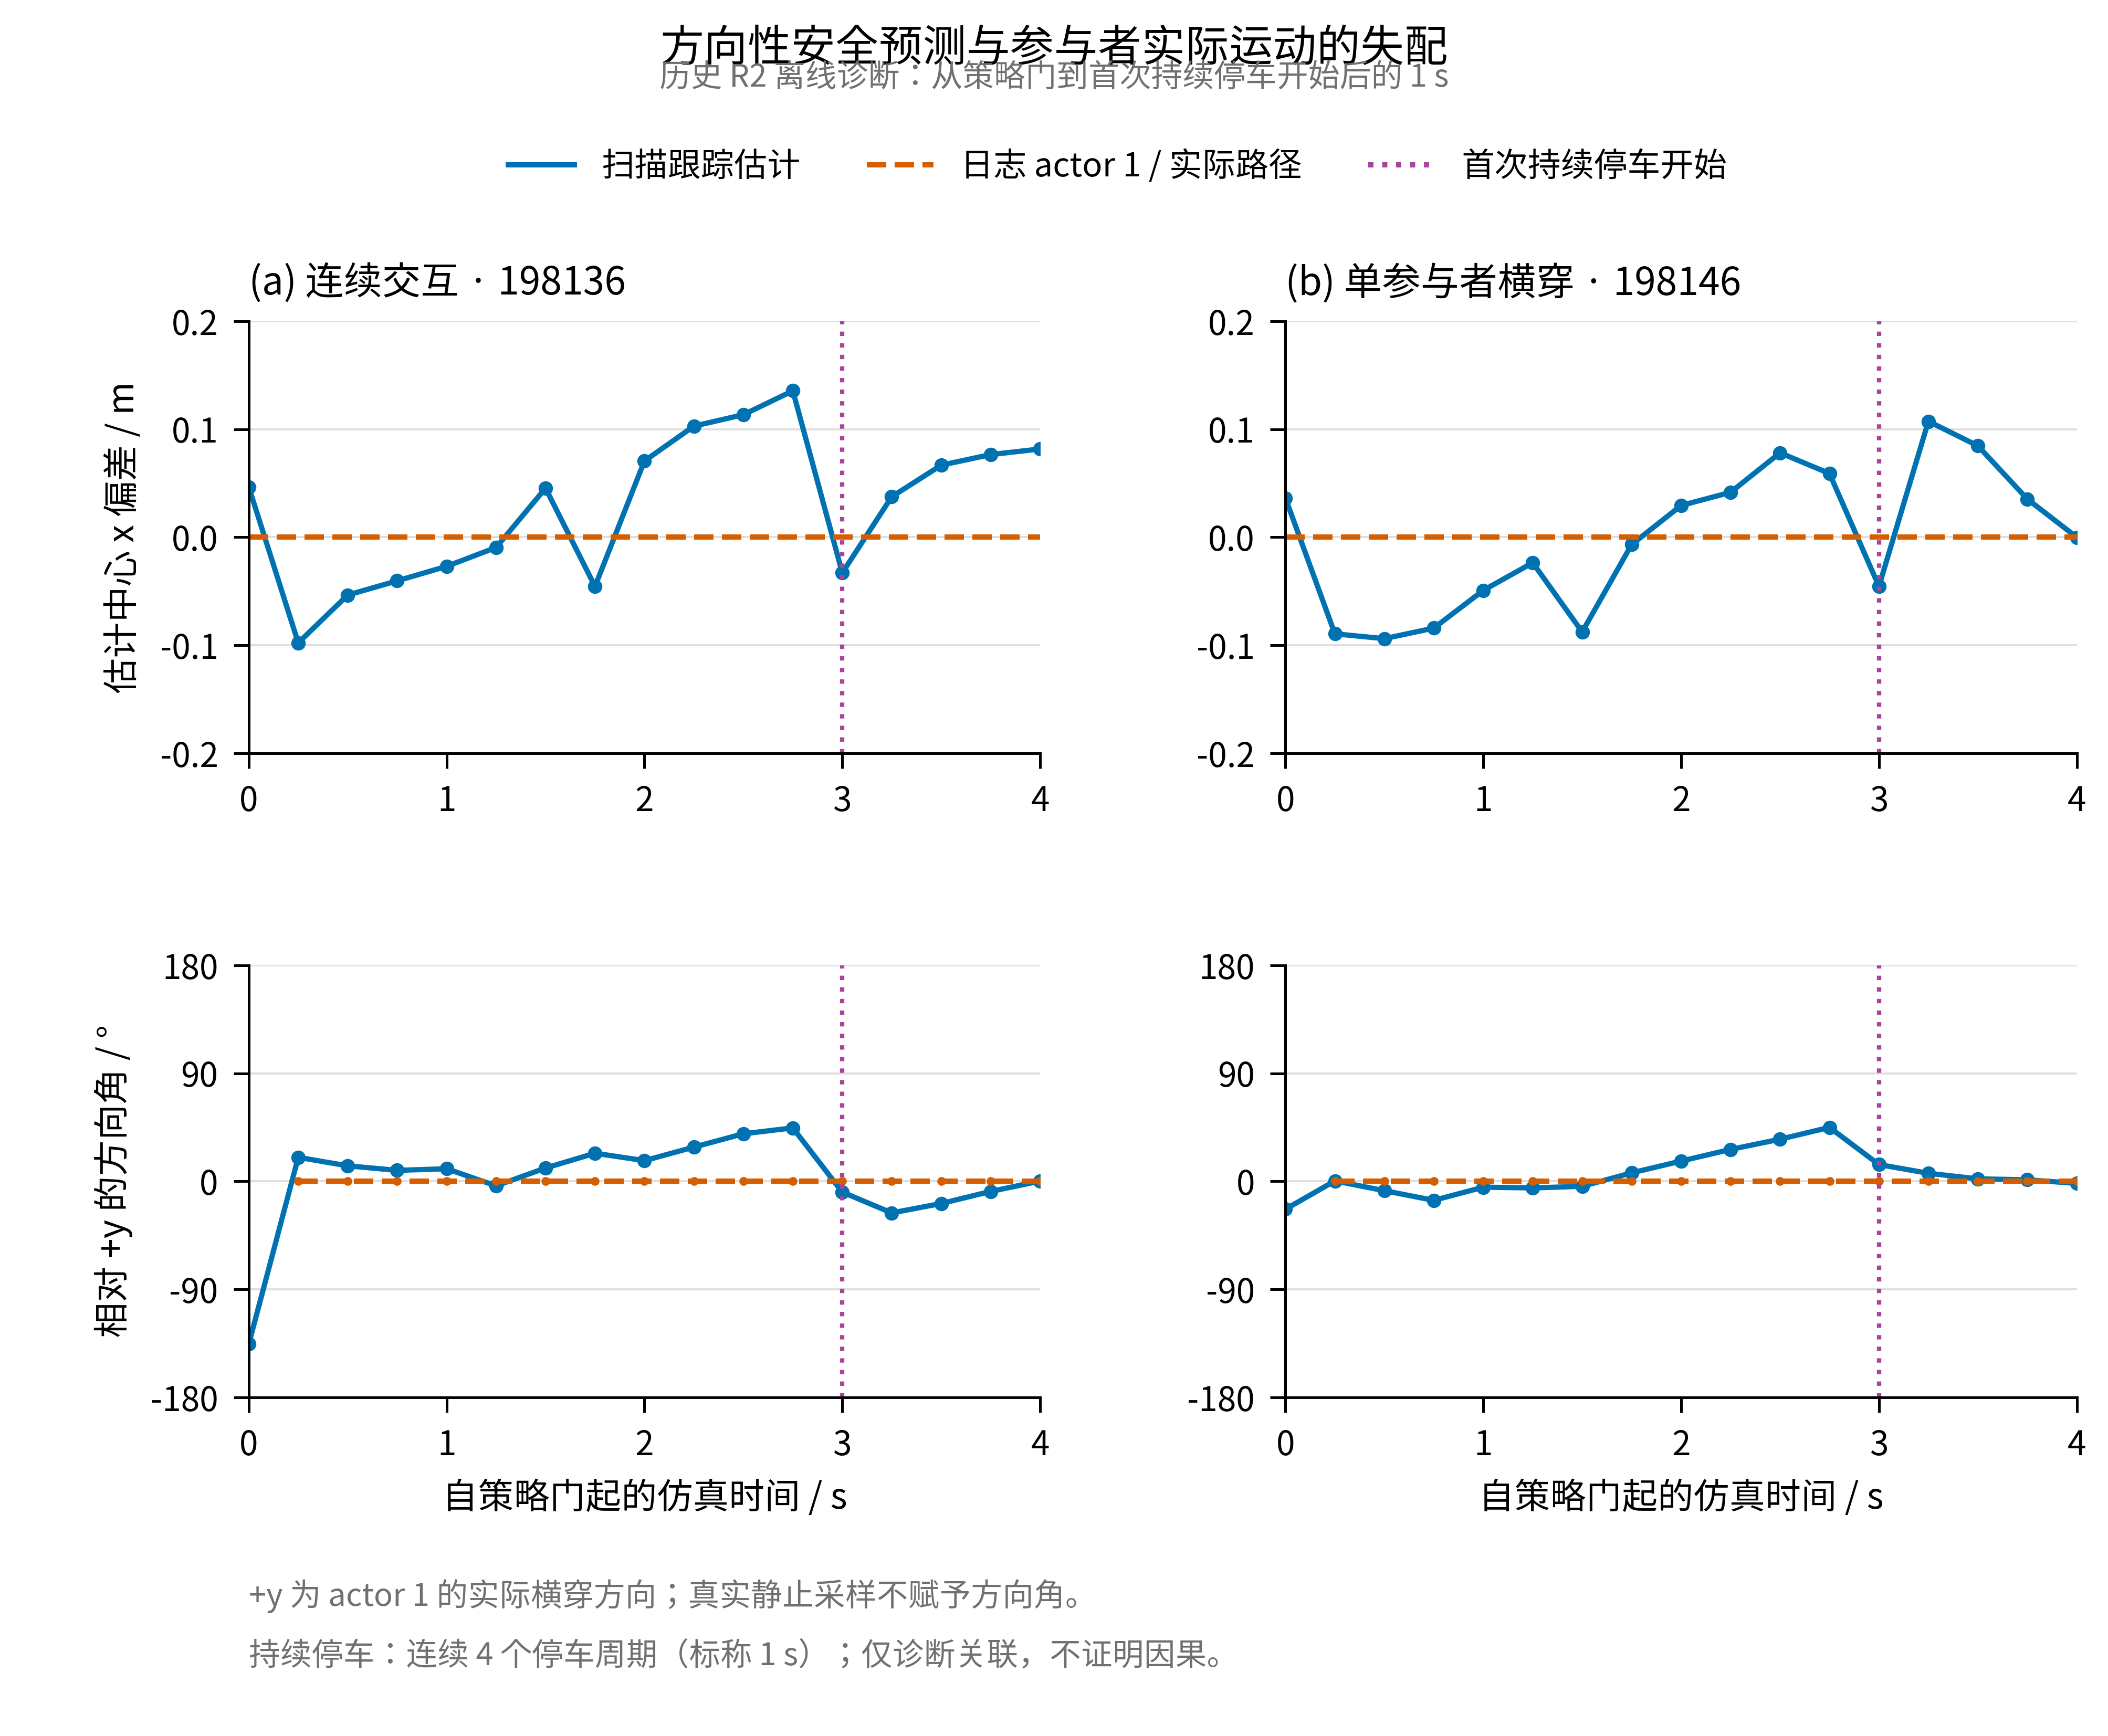
\includegraphics[width=\linewidth]{artifacts/astra_gazebo_20260926/visuals/plots/historical_diagnosis/r03/H02.png}
  \caption{方向性负全预测失配。方向性预测与参与者实际运动如何偏离}
  \label{fig:astra-h02}
\end{figure}

\begin{figure}[tbp]
  \centering
  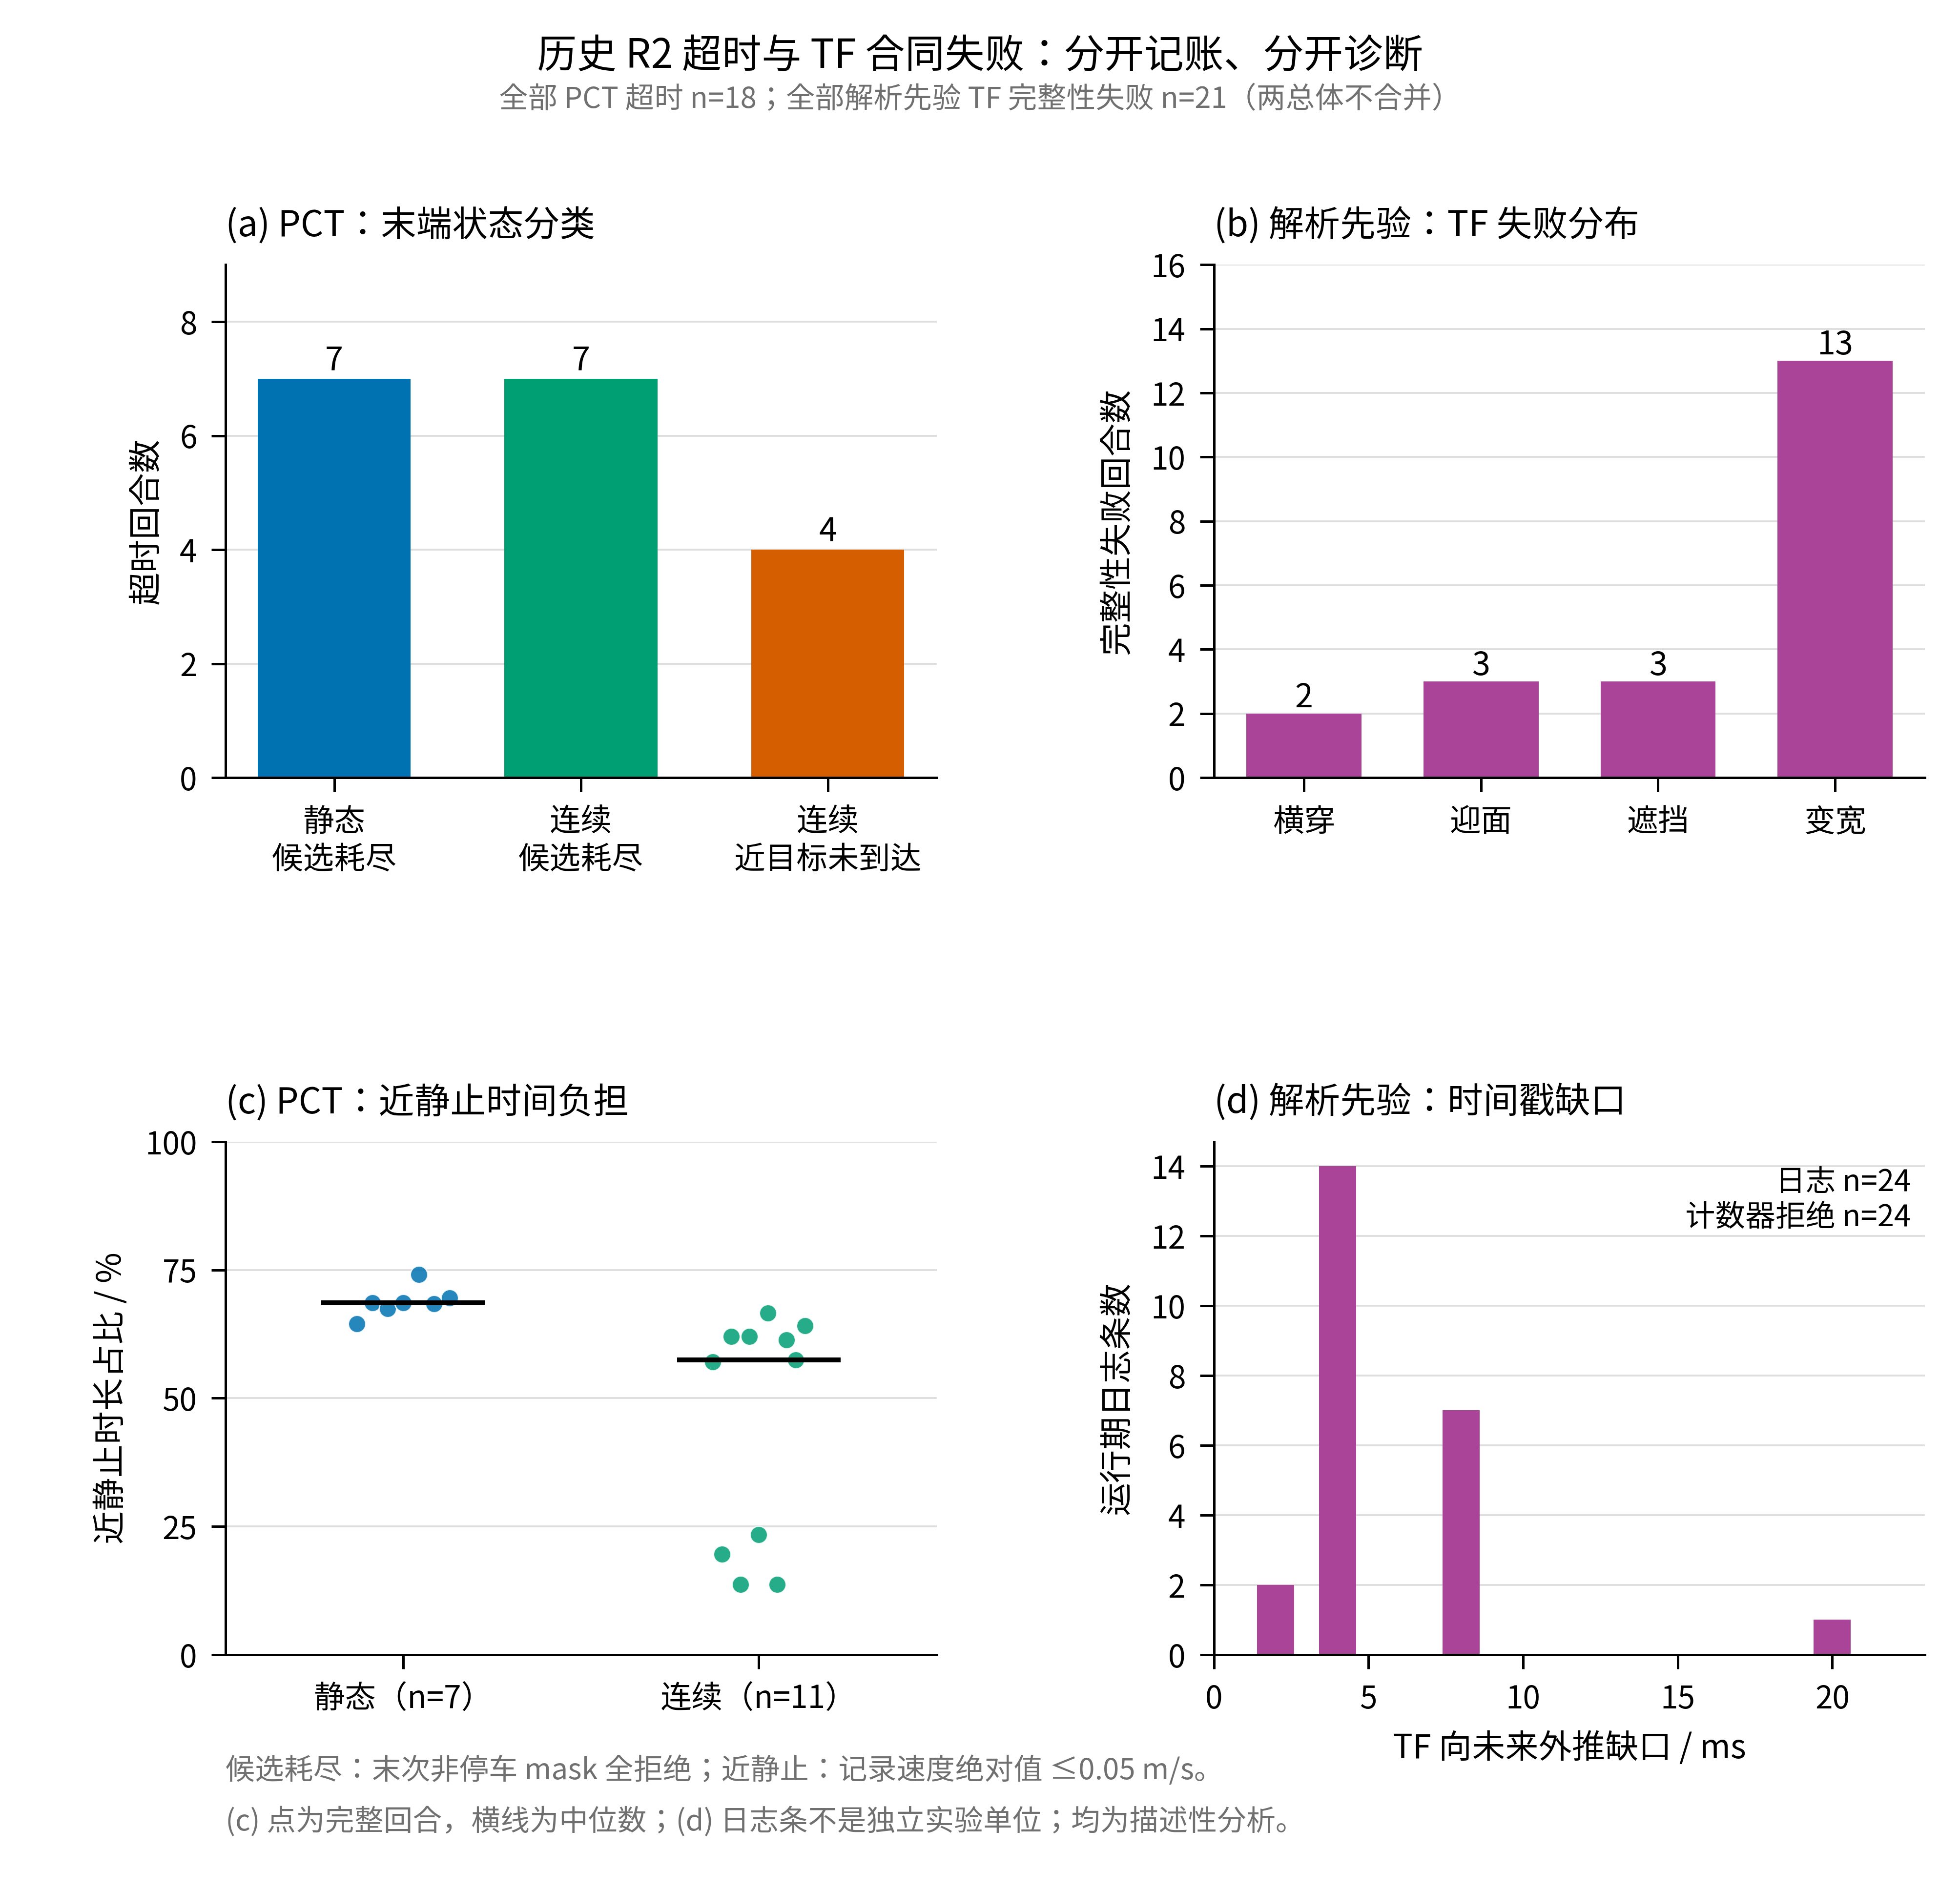
\includegraphics[width=\linewidth]{artifacts/astra_gazebo_20260926/visuals/plots/historical_diagnosis/r03/H03.png}
  \caption{历史超时与 TF 失败分账。超时和 TF 失败应如何独立记录}
  \label{fig:astra-h03}
\end{figure}

\begin{figure}[tbp]
  \centering
  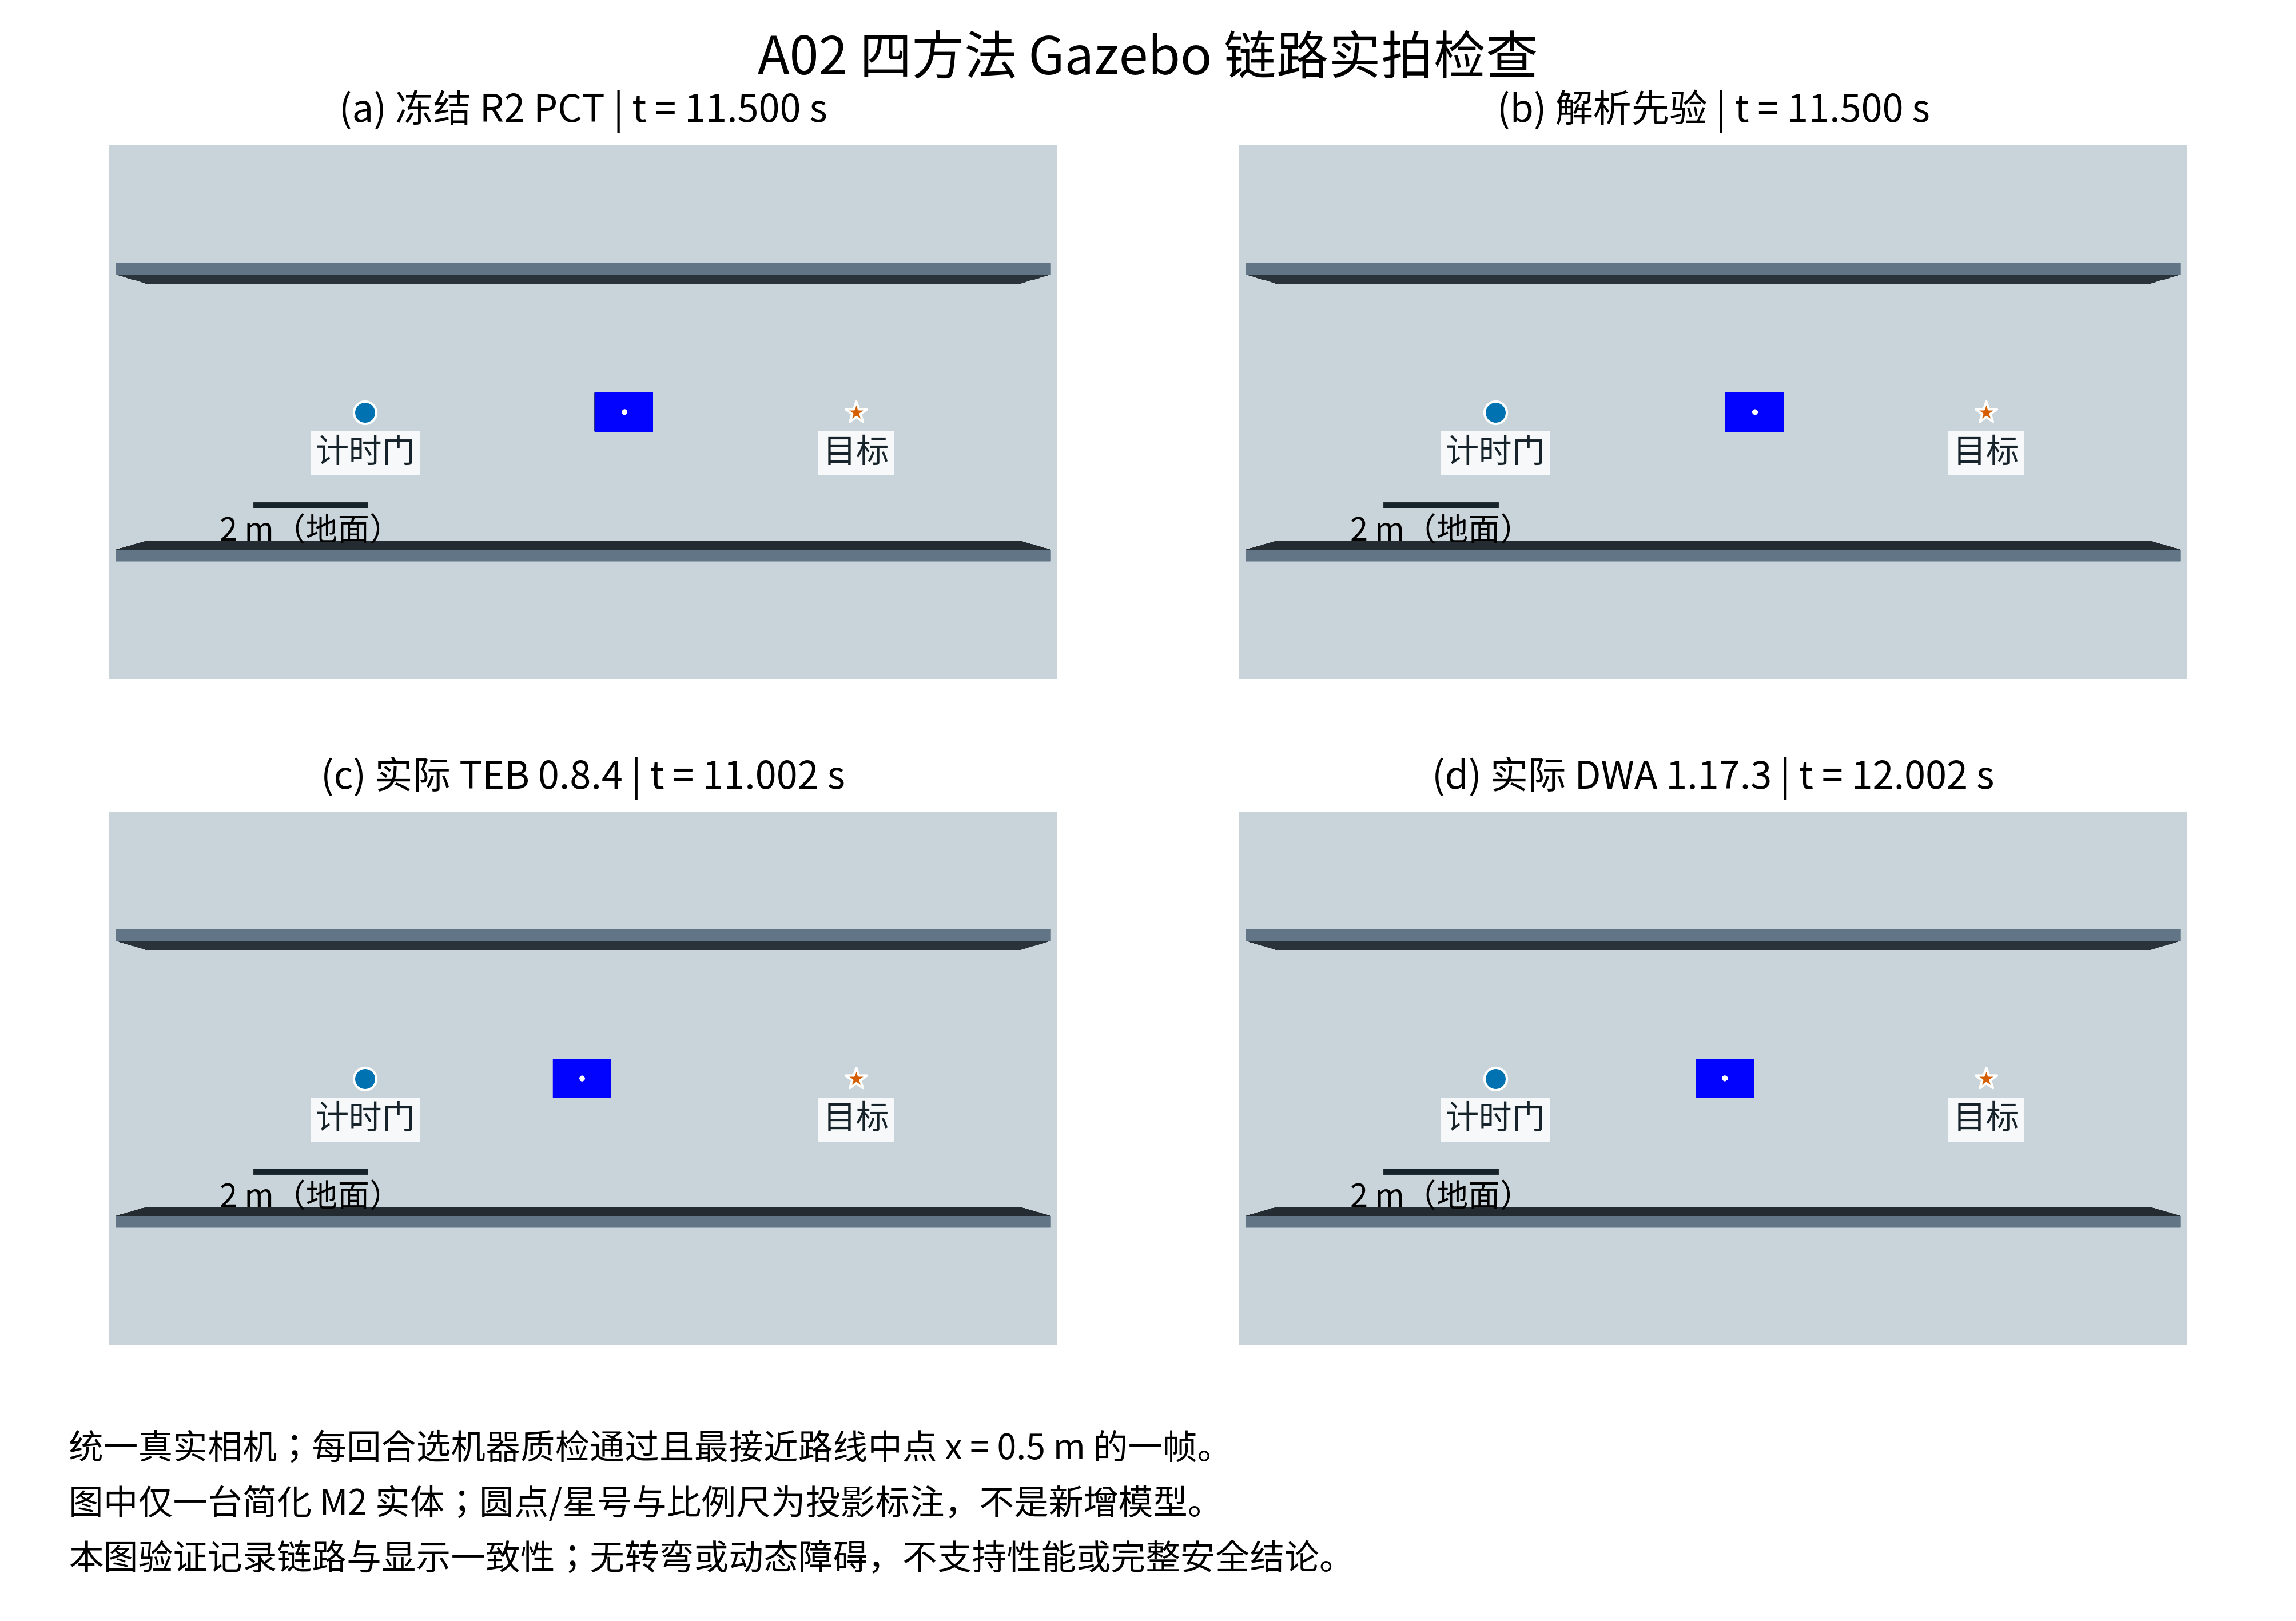
\includegraphics[width=\linewidth]{artifacts/astra_gazebo_20260926/visuals/panels/bootstrap_a02/r01/Q01_smoke_overview.png}
  \caption{四方法 Gazebo 链路实拍检查。四个方法的早期 Gazebo 图像链路是否形成}
  \label{fig:astra-q01}
\end{figure}

\begin{figure}[tbp]
  \centering
  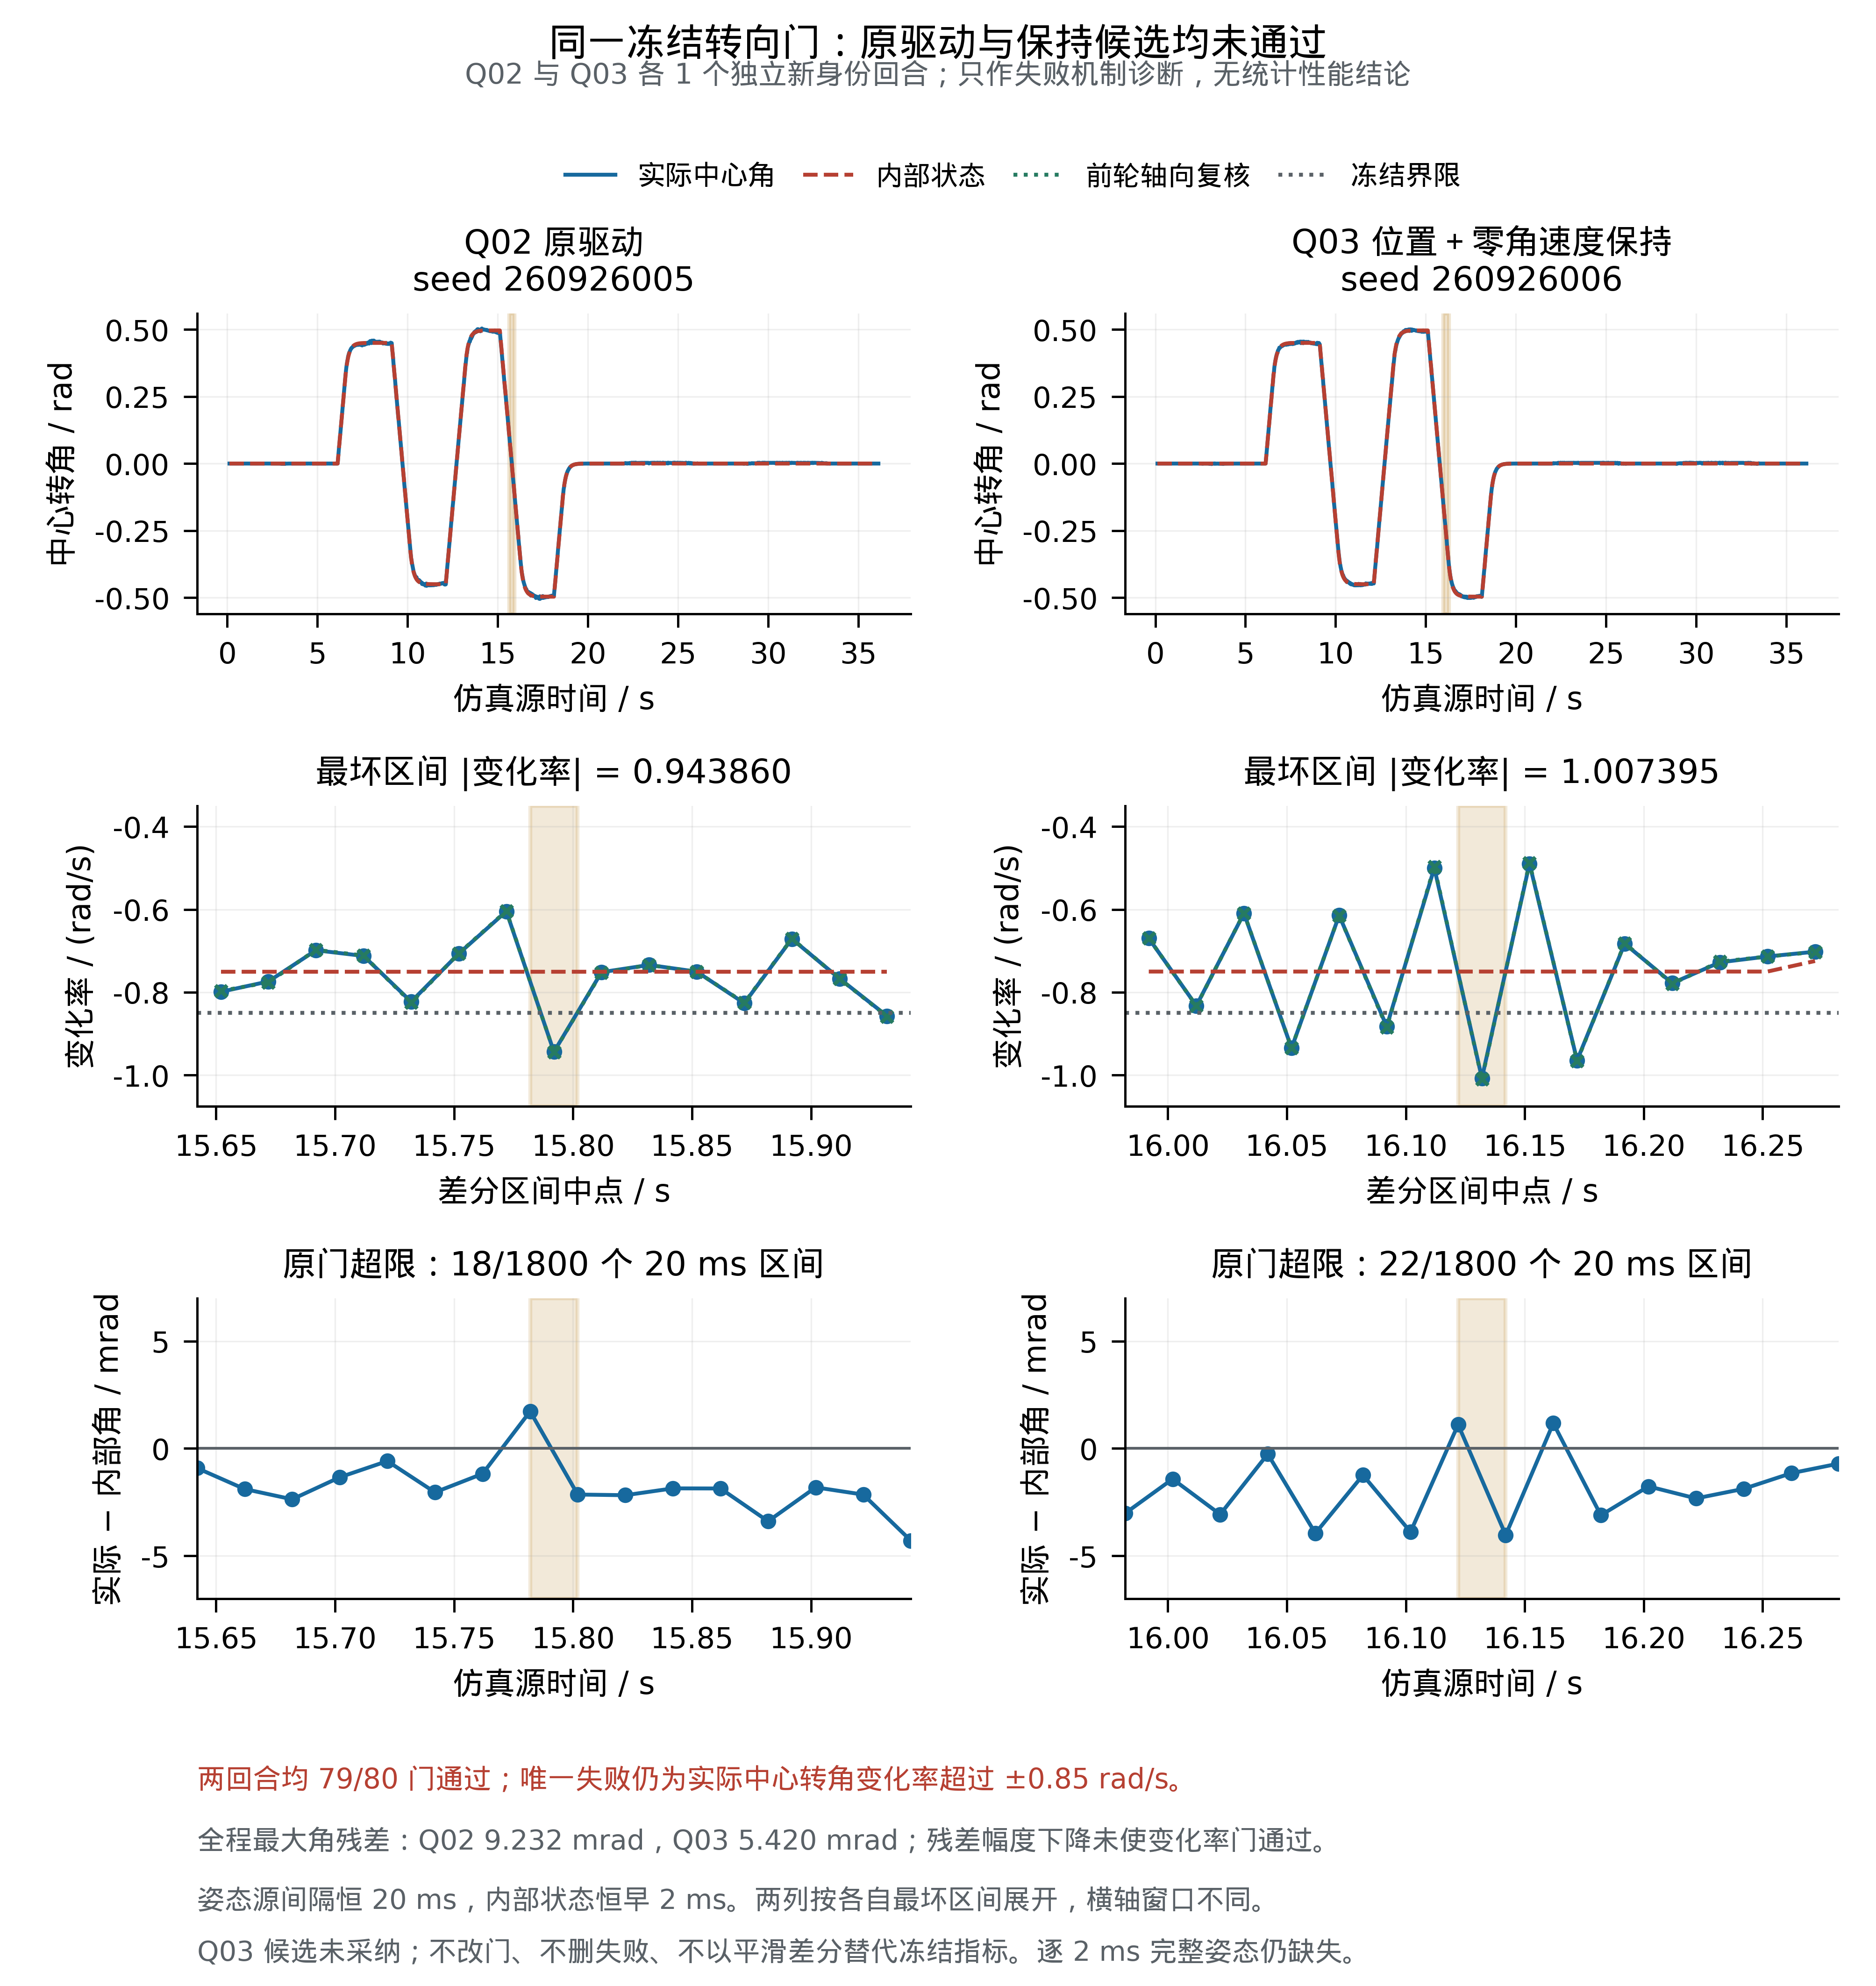
\includegraphics[width=\linewidth]{artifacts/astra_gazebo_20260926/visuals/plots/actuation_q03_comparison/r02/AQC02.png}
  \caption{冻结转向门下的驱动比较。原驱动与假转速通道在同一转向门下如何表现}
  \label{fig:astra-aqc02}
\end{figure}

\begin{figure}[tbp]
  \centering
  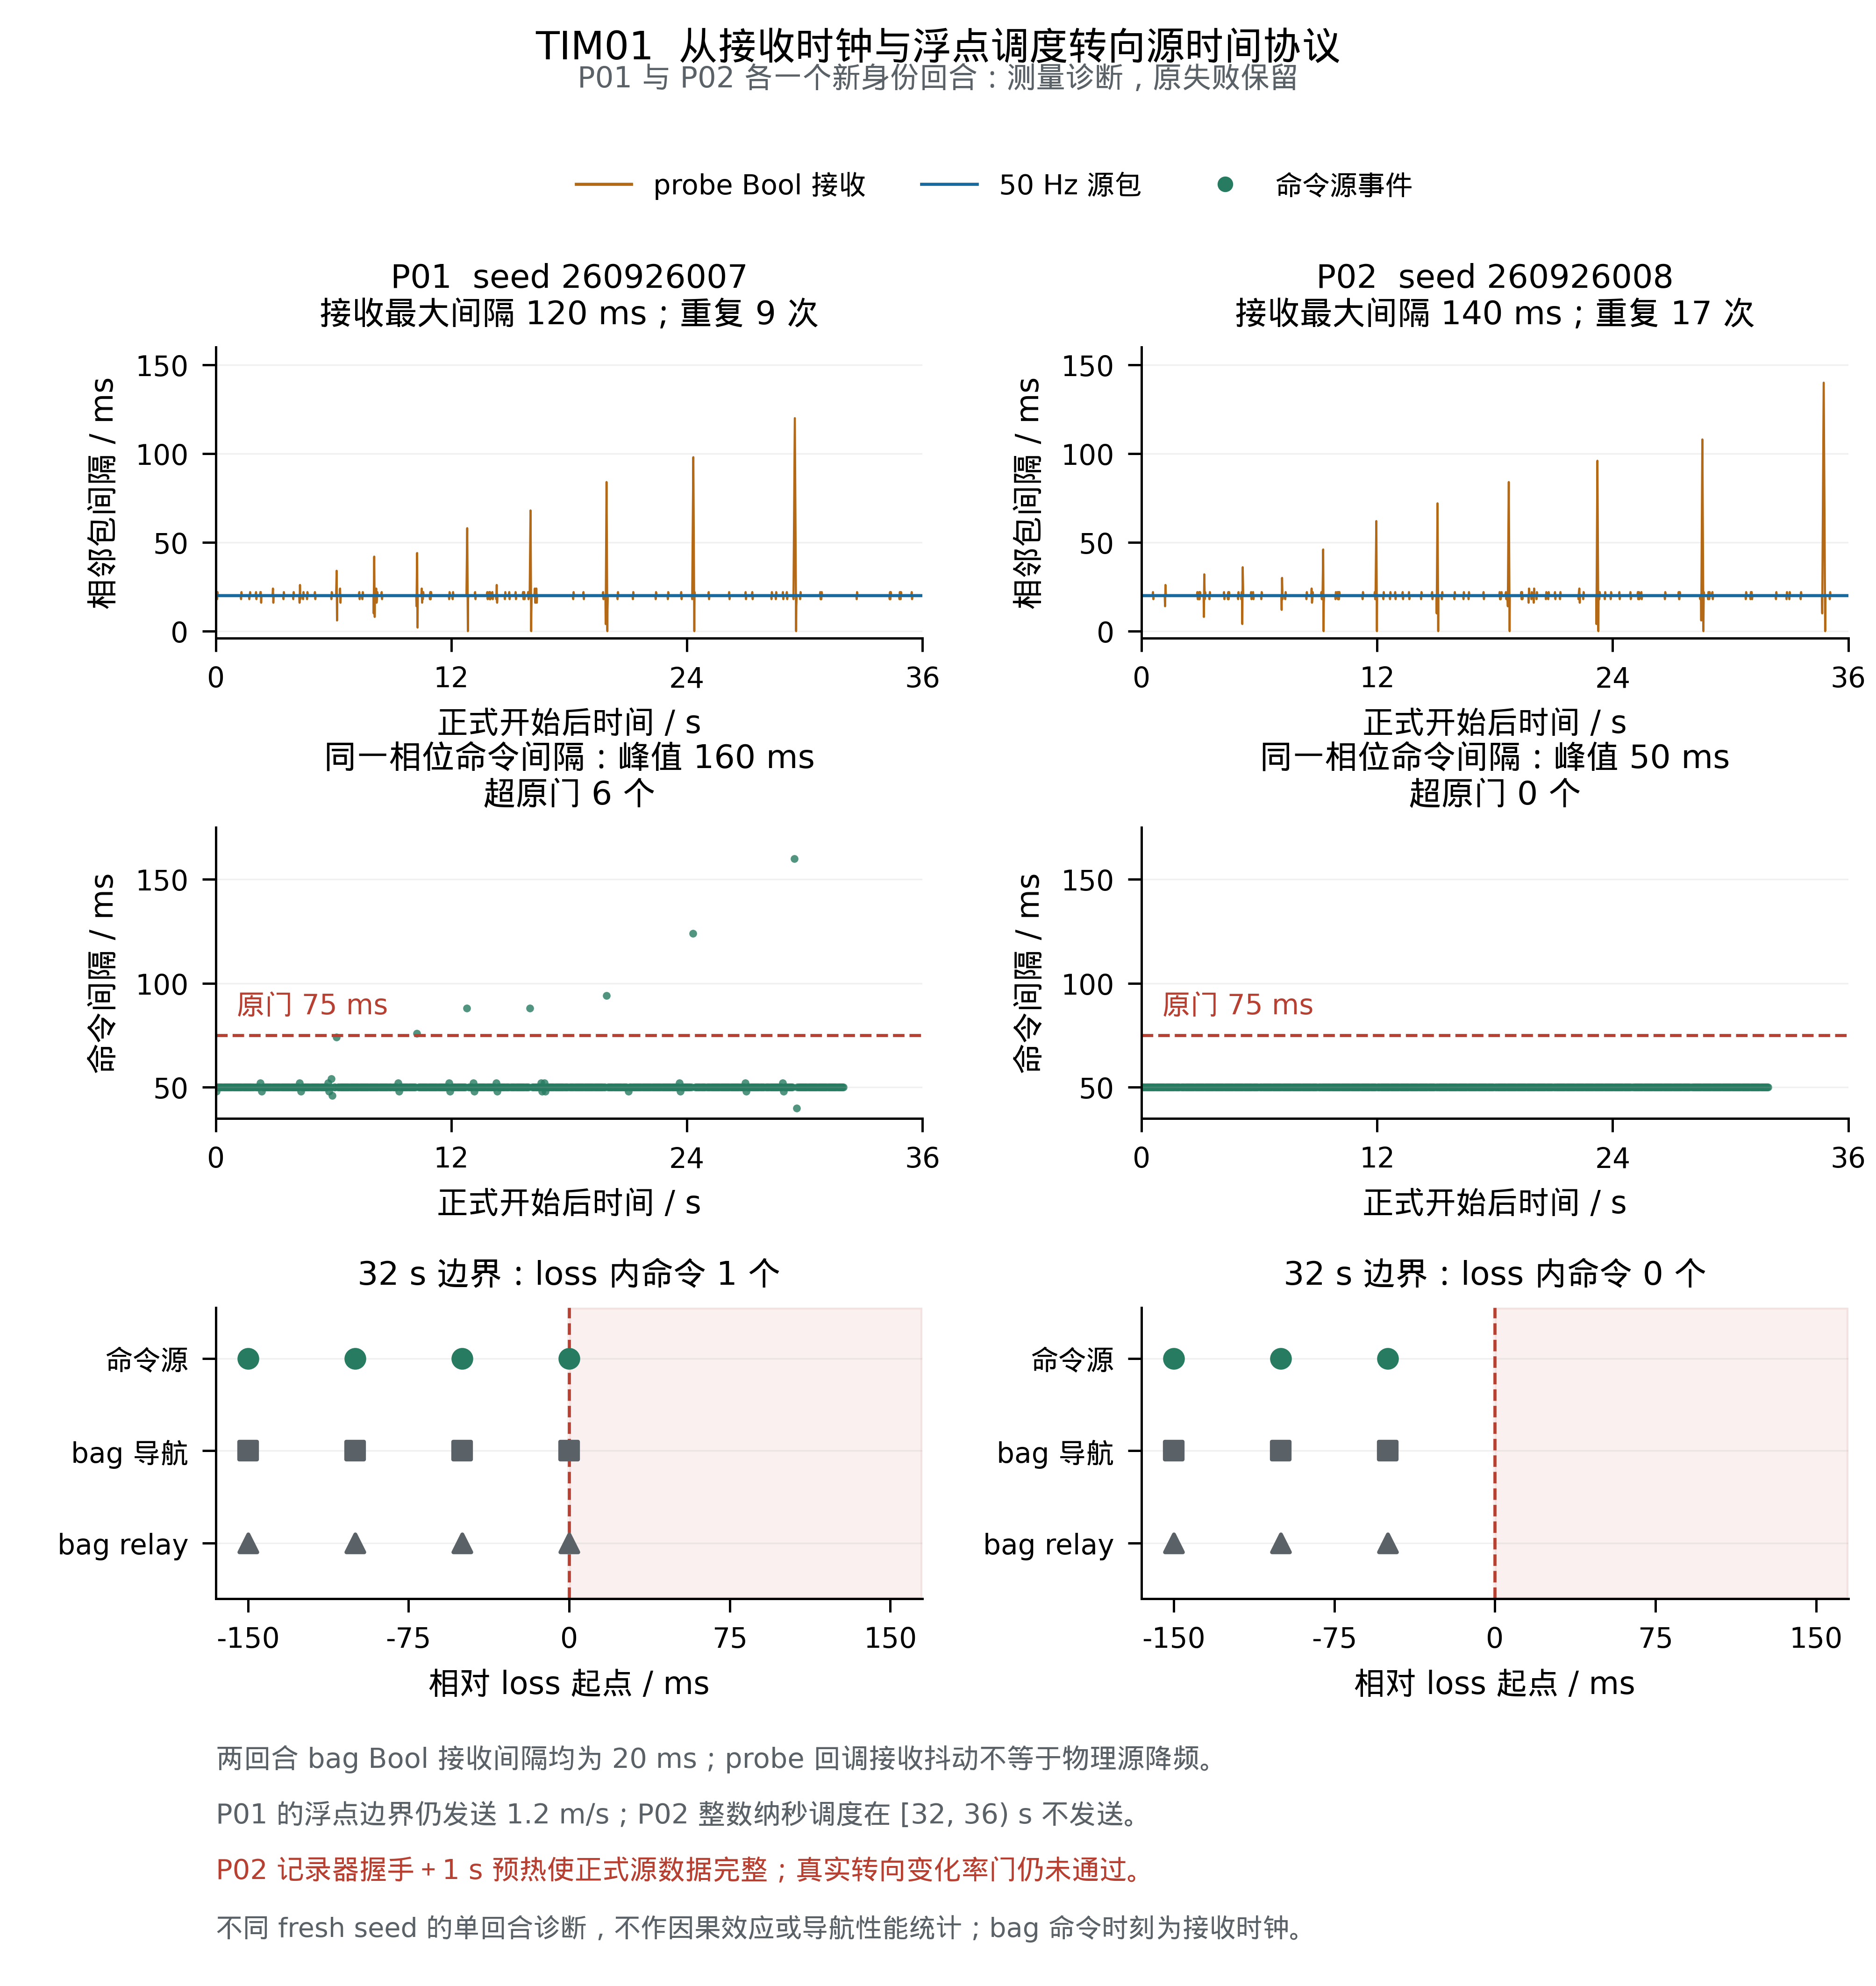
\includegraphics[width=\linewidth]{artifacts/astra_gazebo_20260926/visuals/plots/physical_qualification/r02/TIM01.png}
  \caption{源时间与异步采集协议。接收时钟和异步采集如何保持时间可追溯}
  \label{fig:astra-tim01}
\end{figure}

\begin{figure}[tbp]
  \centering
  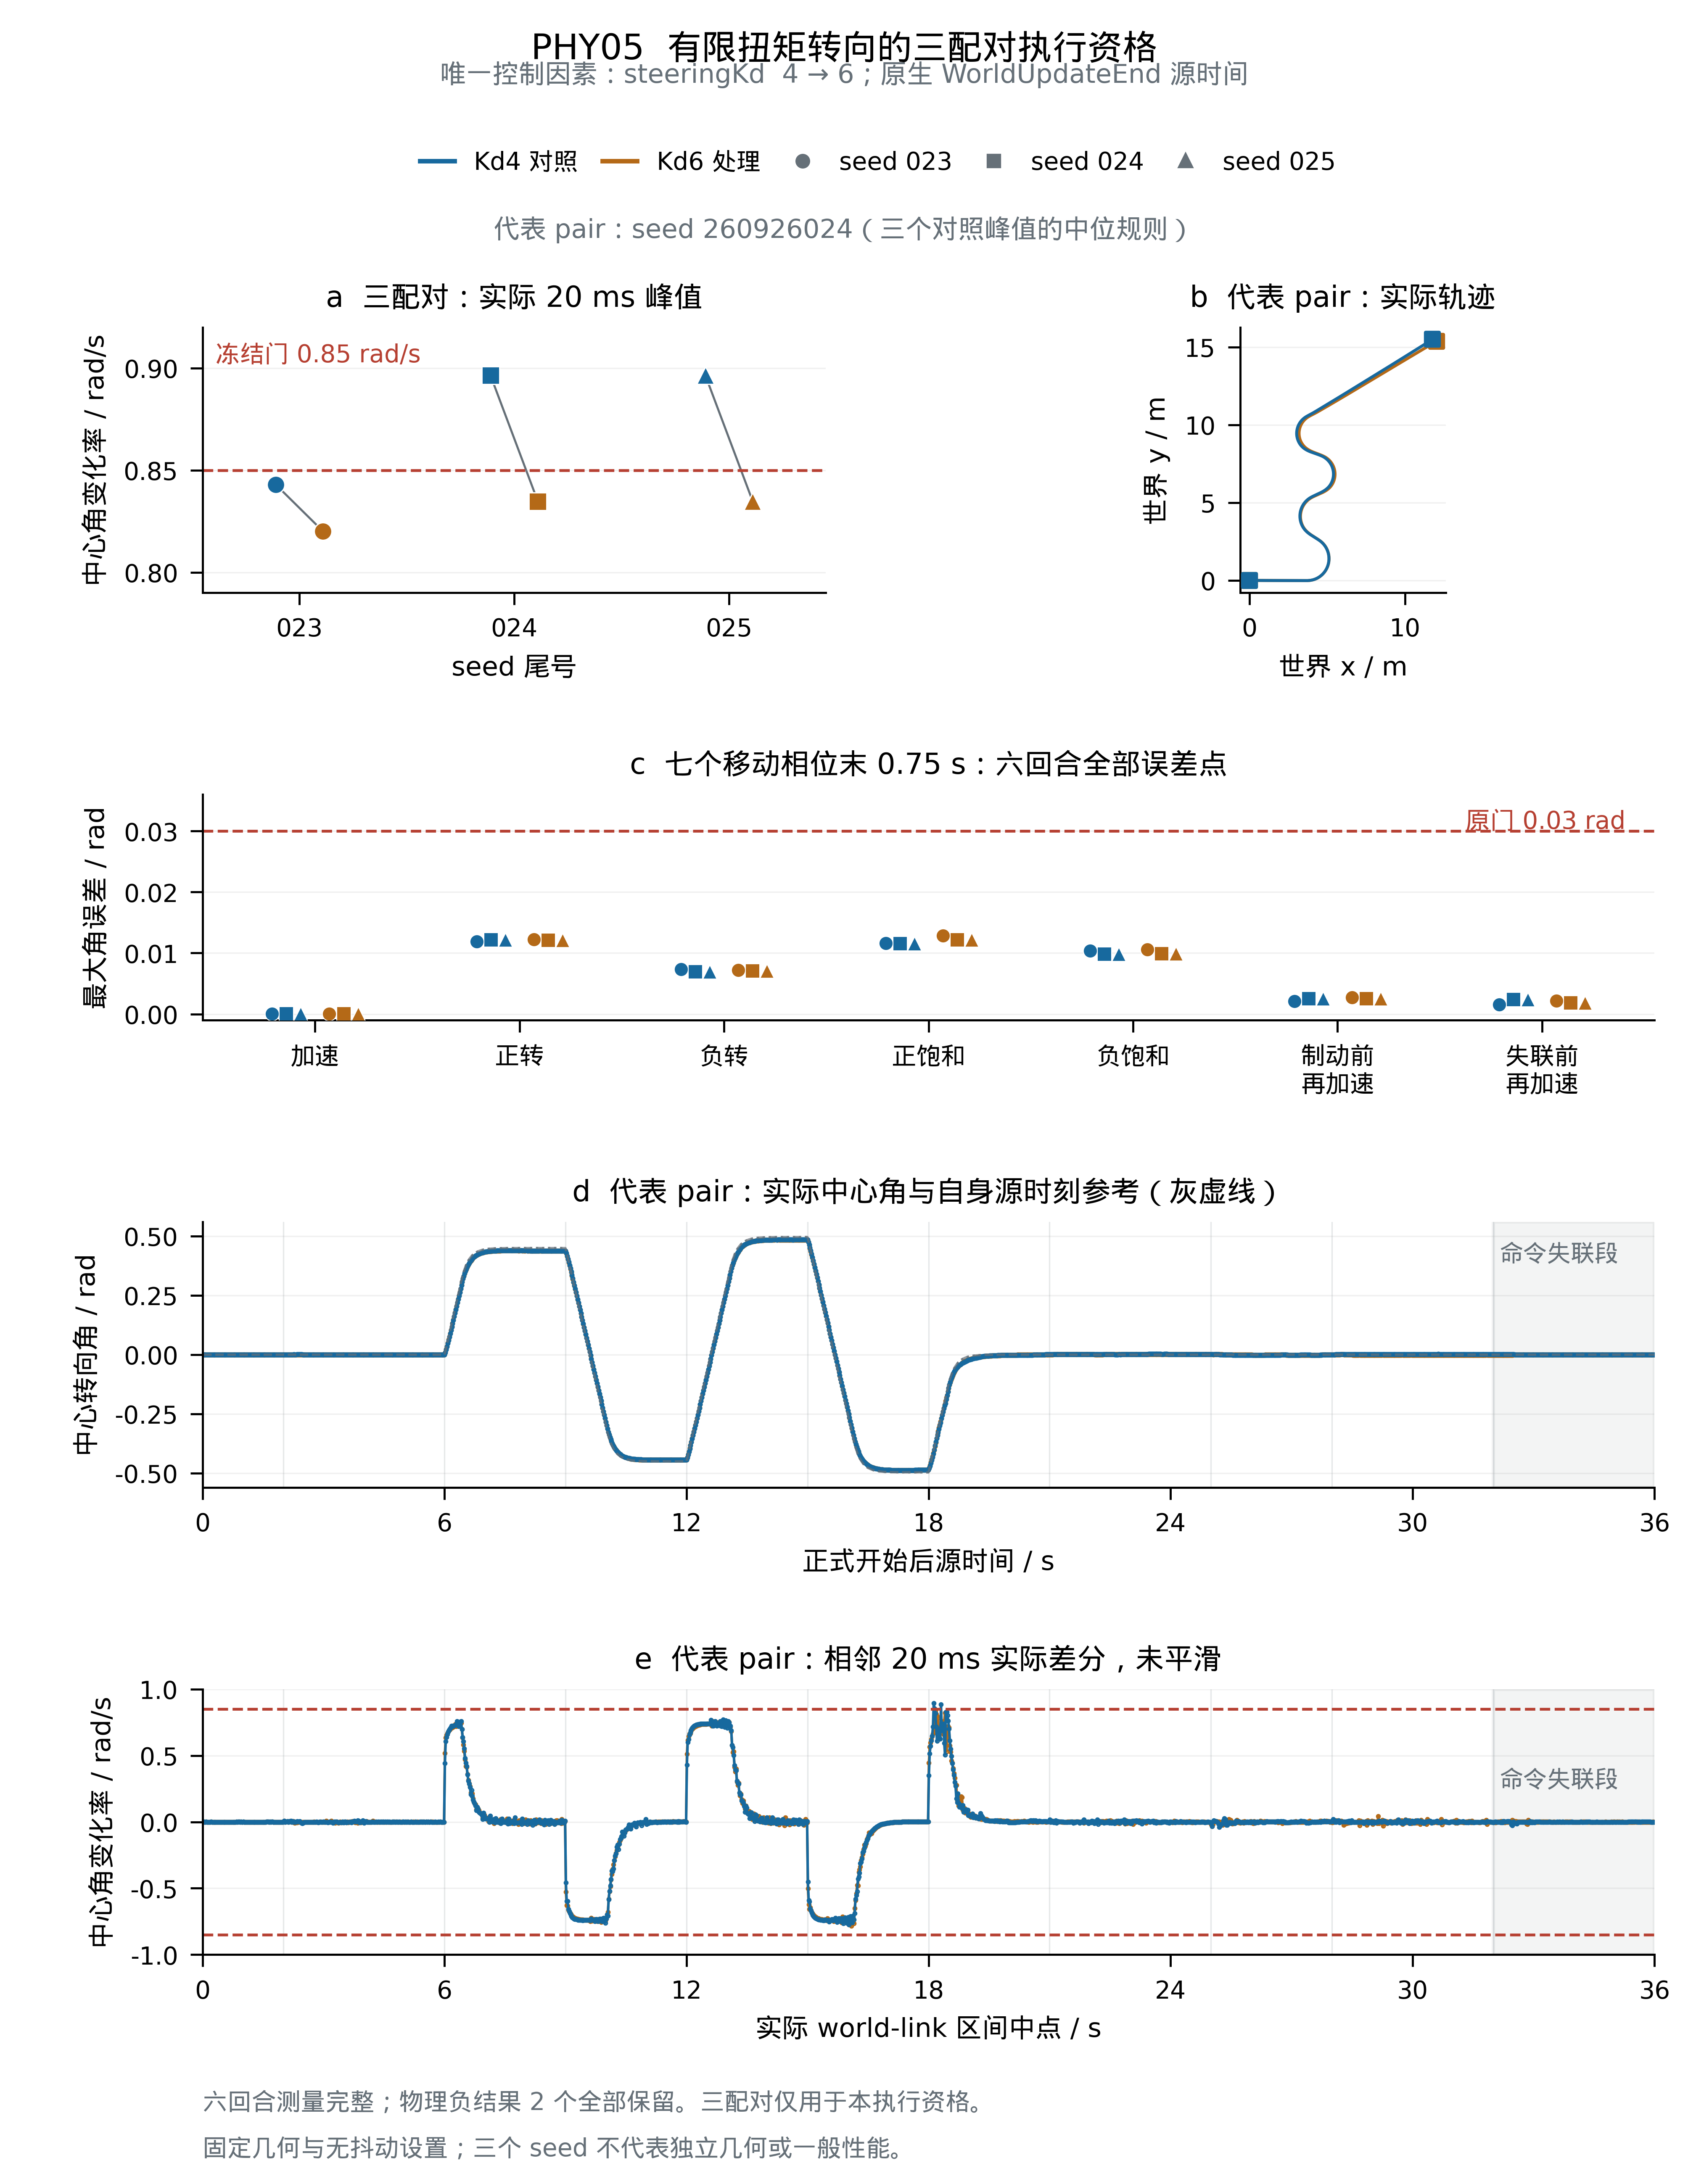
\includegraphics[width=\linewidth]{artifacts/astra_gazebo_20260926/visuals/plots/physical_qualification/PHY05/r03/PHY05.png}
  \caption{有界转向半径的三阶段执行。三阶段转向执行能否形成连续物理轨迹}
  \label{fig:astra-phy05}
\end{figure}

\begin{figure}[tbp]
  \centering
  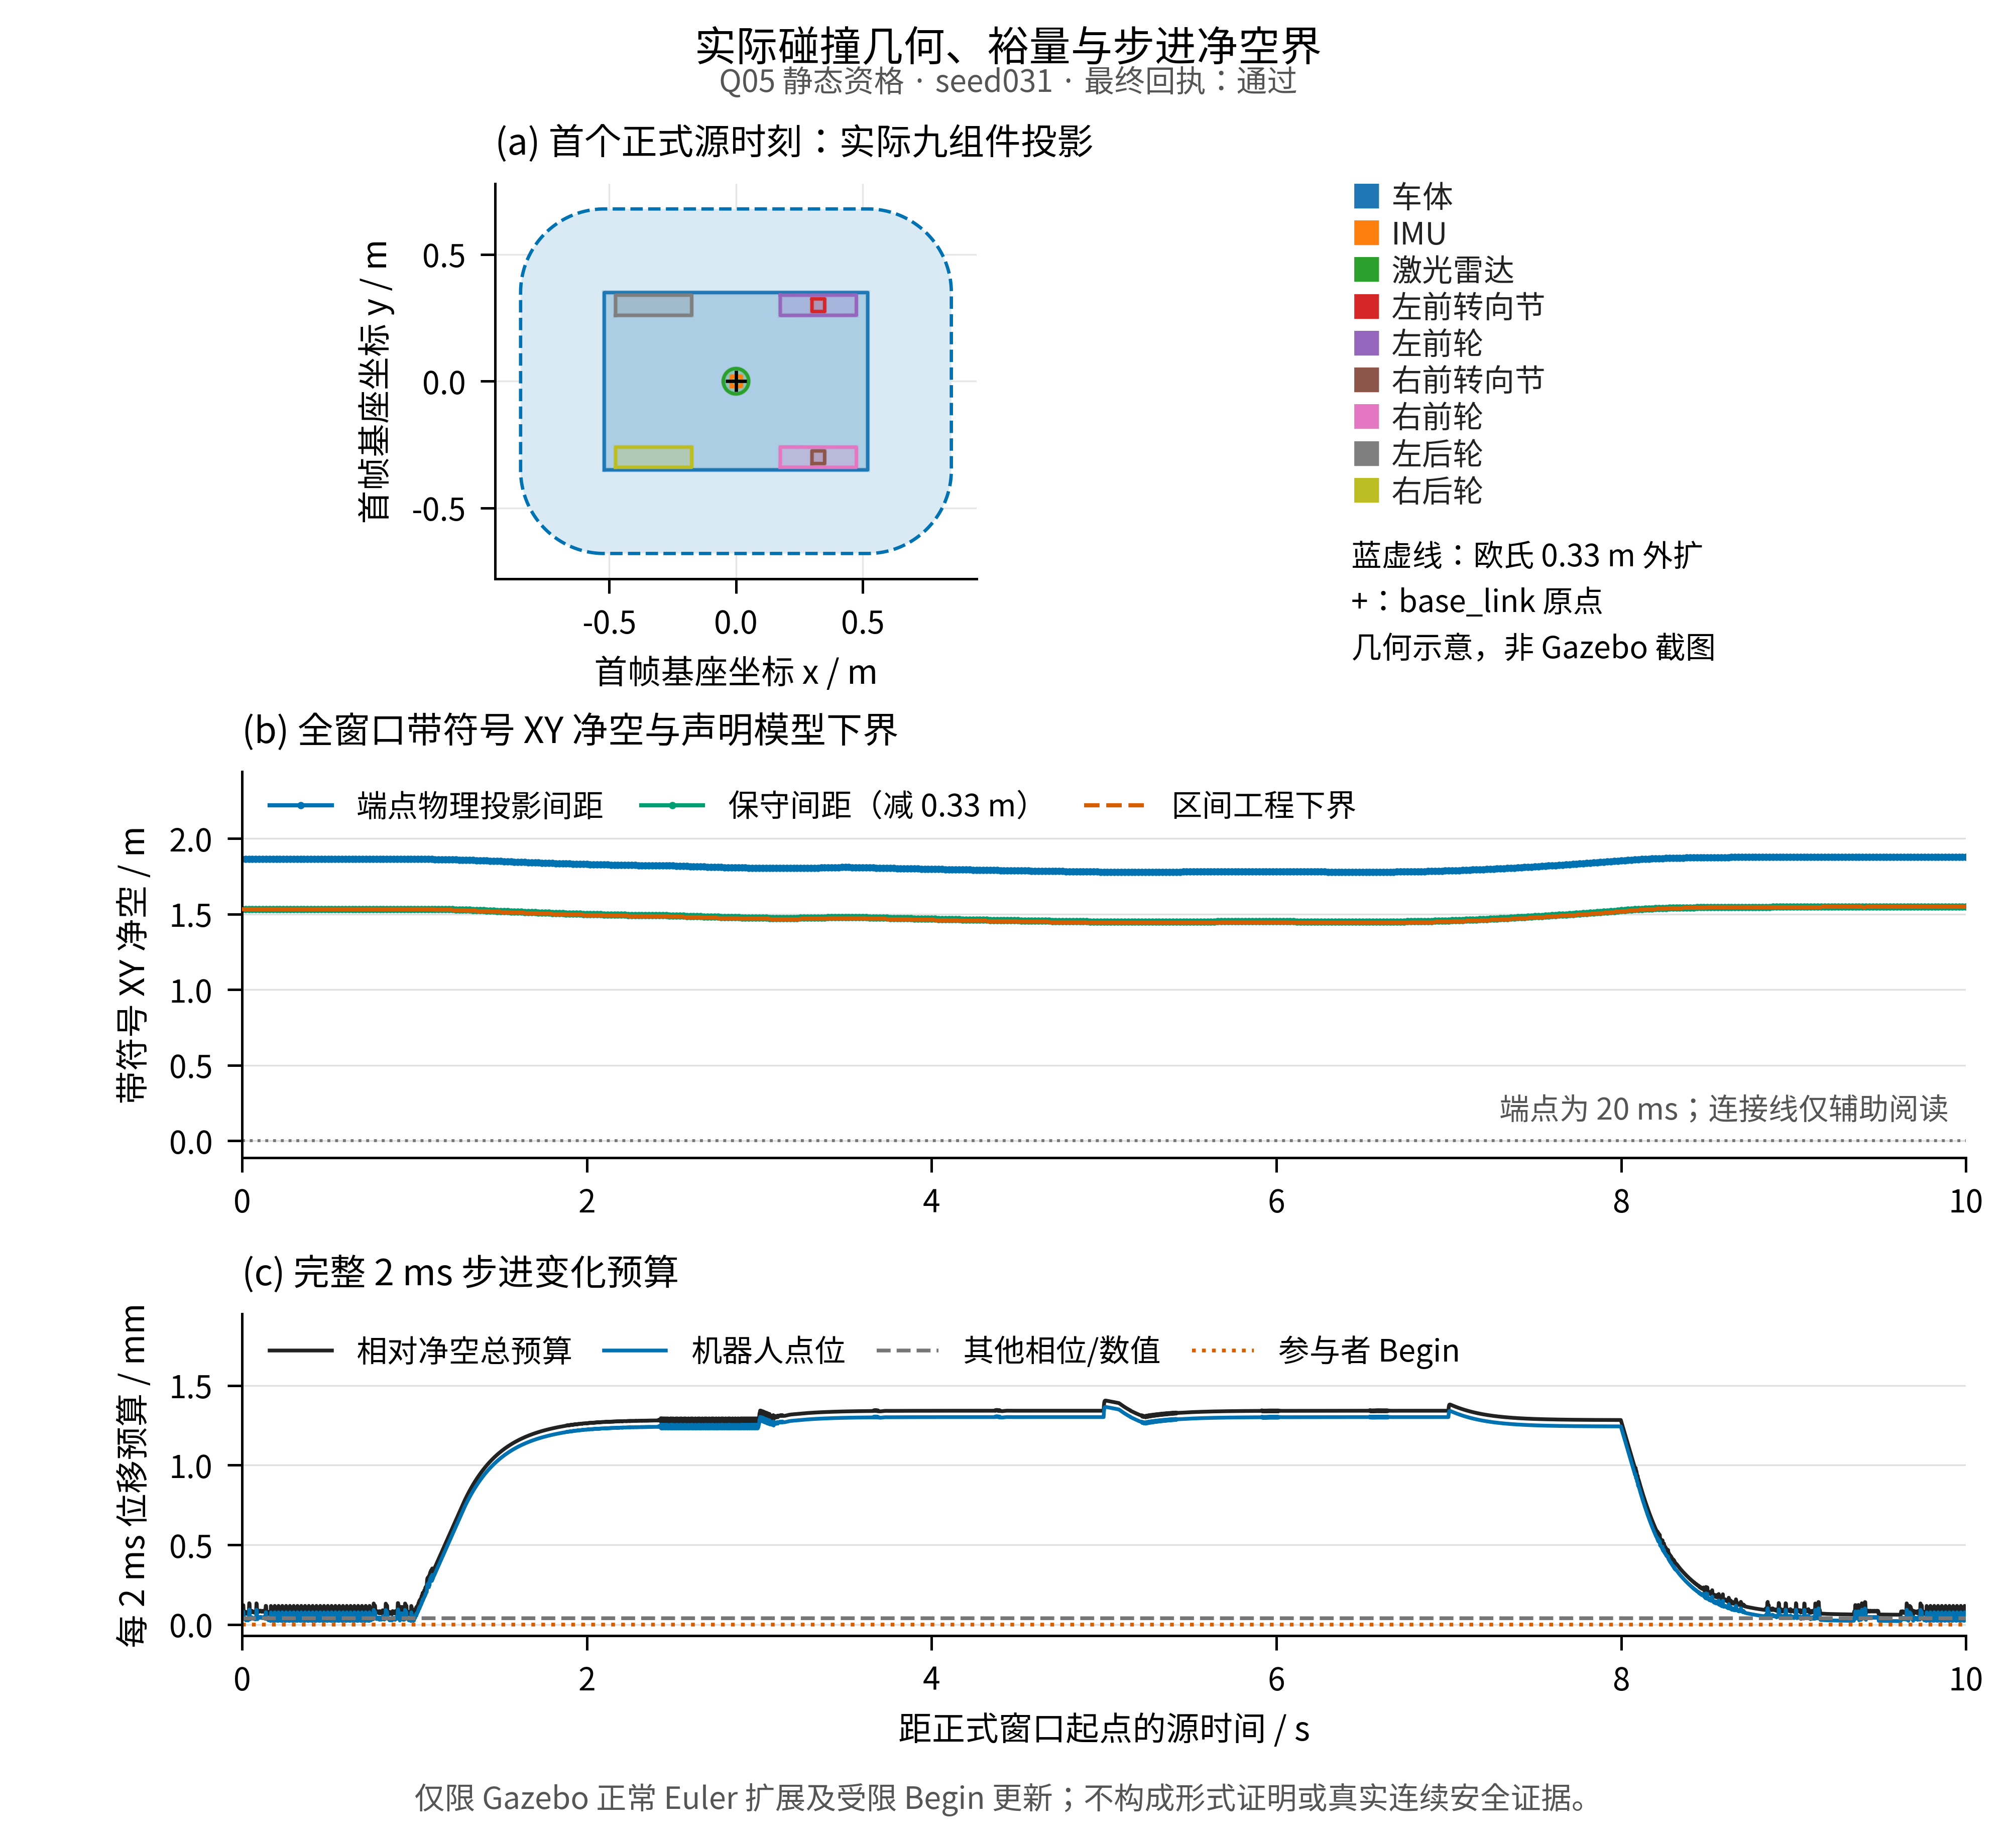
\includegraphics[width=\linewidth]{artifacts/astra_gazebo_20260926/visuals/plots/geometry_contract/r07/F04.png}
  \caption{物理与保守净空。方盒和机器人compound净空如何定义}
  \label{fig:astra-f04}
\end{figure}

\begin{figure}[tbp]
  \centering
  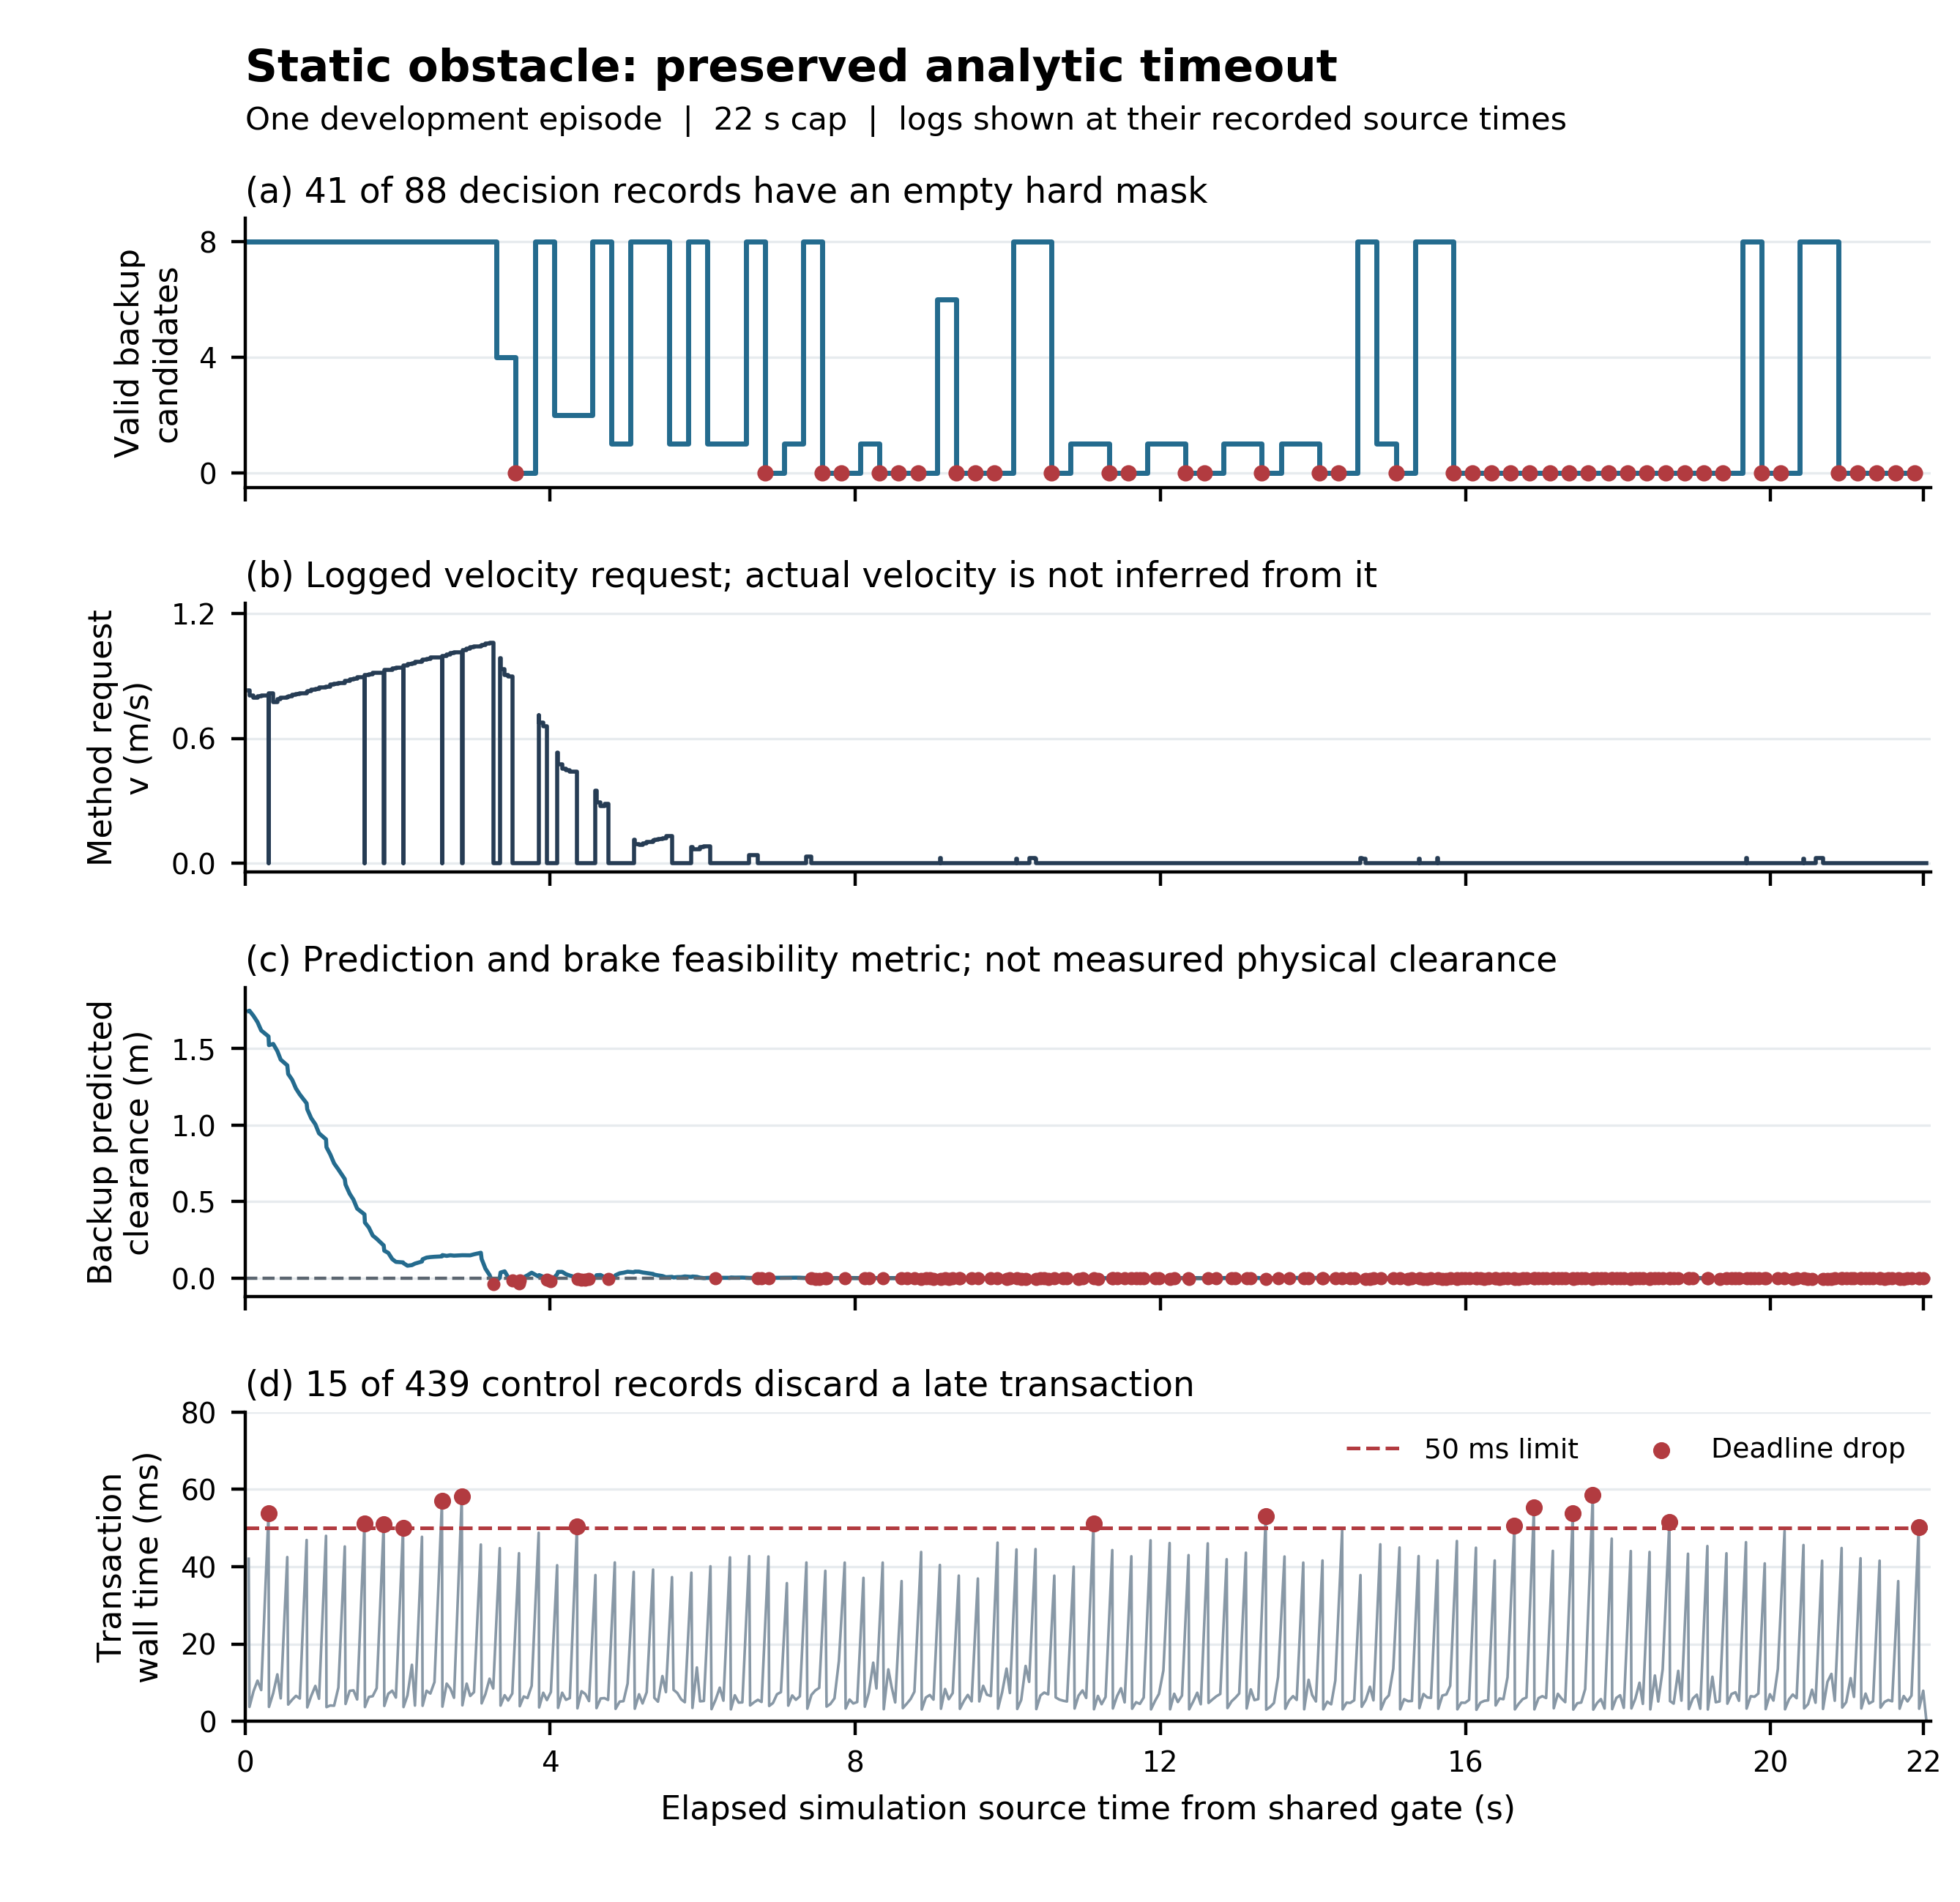
\includegraphics[width=\linewidth]{artifacts/astra_gazebo_20260926/visuals/plots/navigation_n04_failure_trace/r02/NAV01_static_failure_trace.png}
  \caption{静态绕障失败中的候选可行性与控制时限。候选mask耗尽及控制时限如何伴随一次开发超时}
  \label{fig:astra-nav01}
\end{figure}

\begin{figure}[tbp]
  \centering
  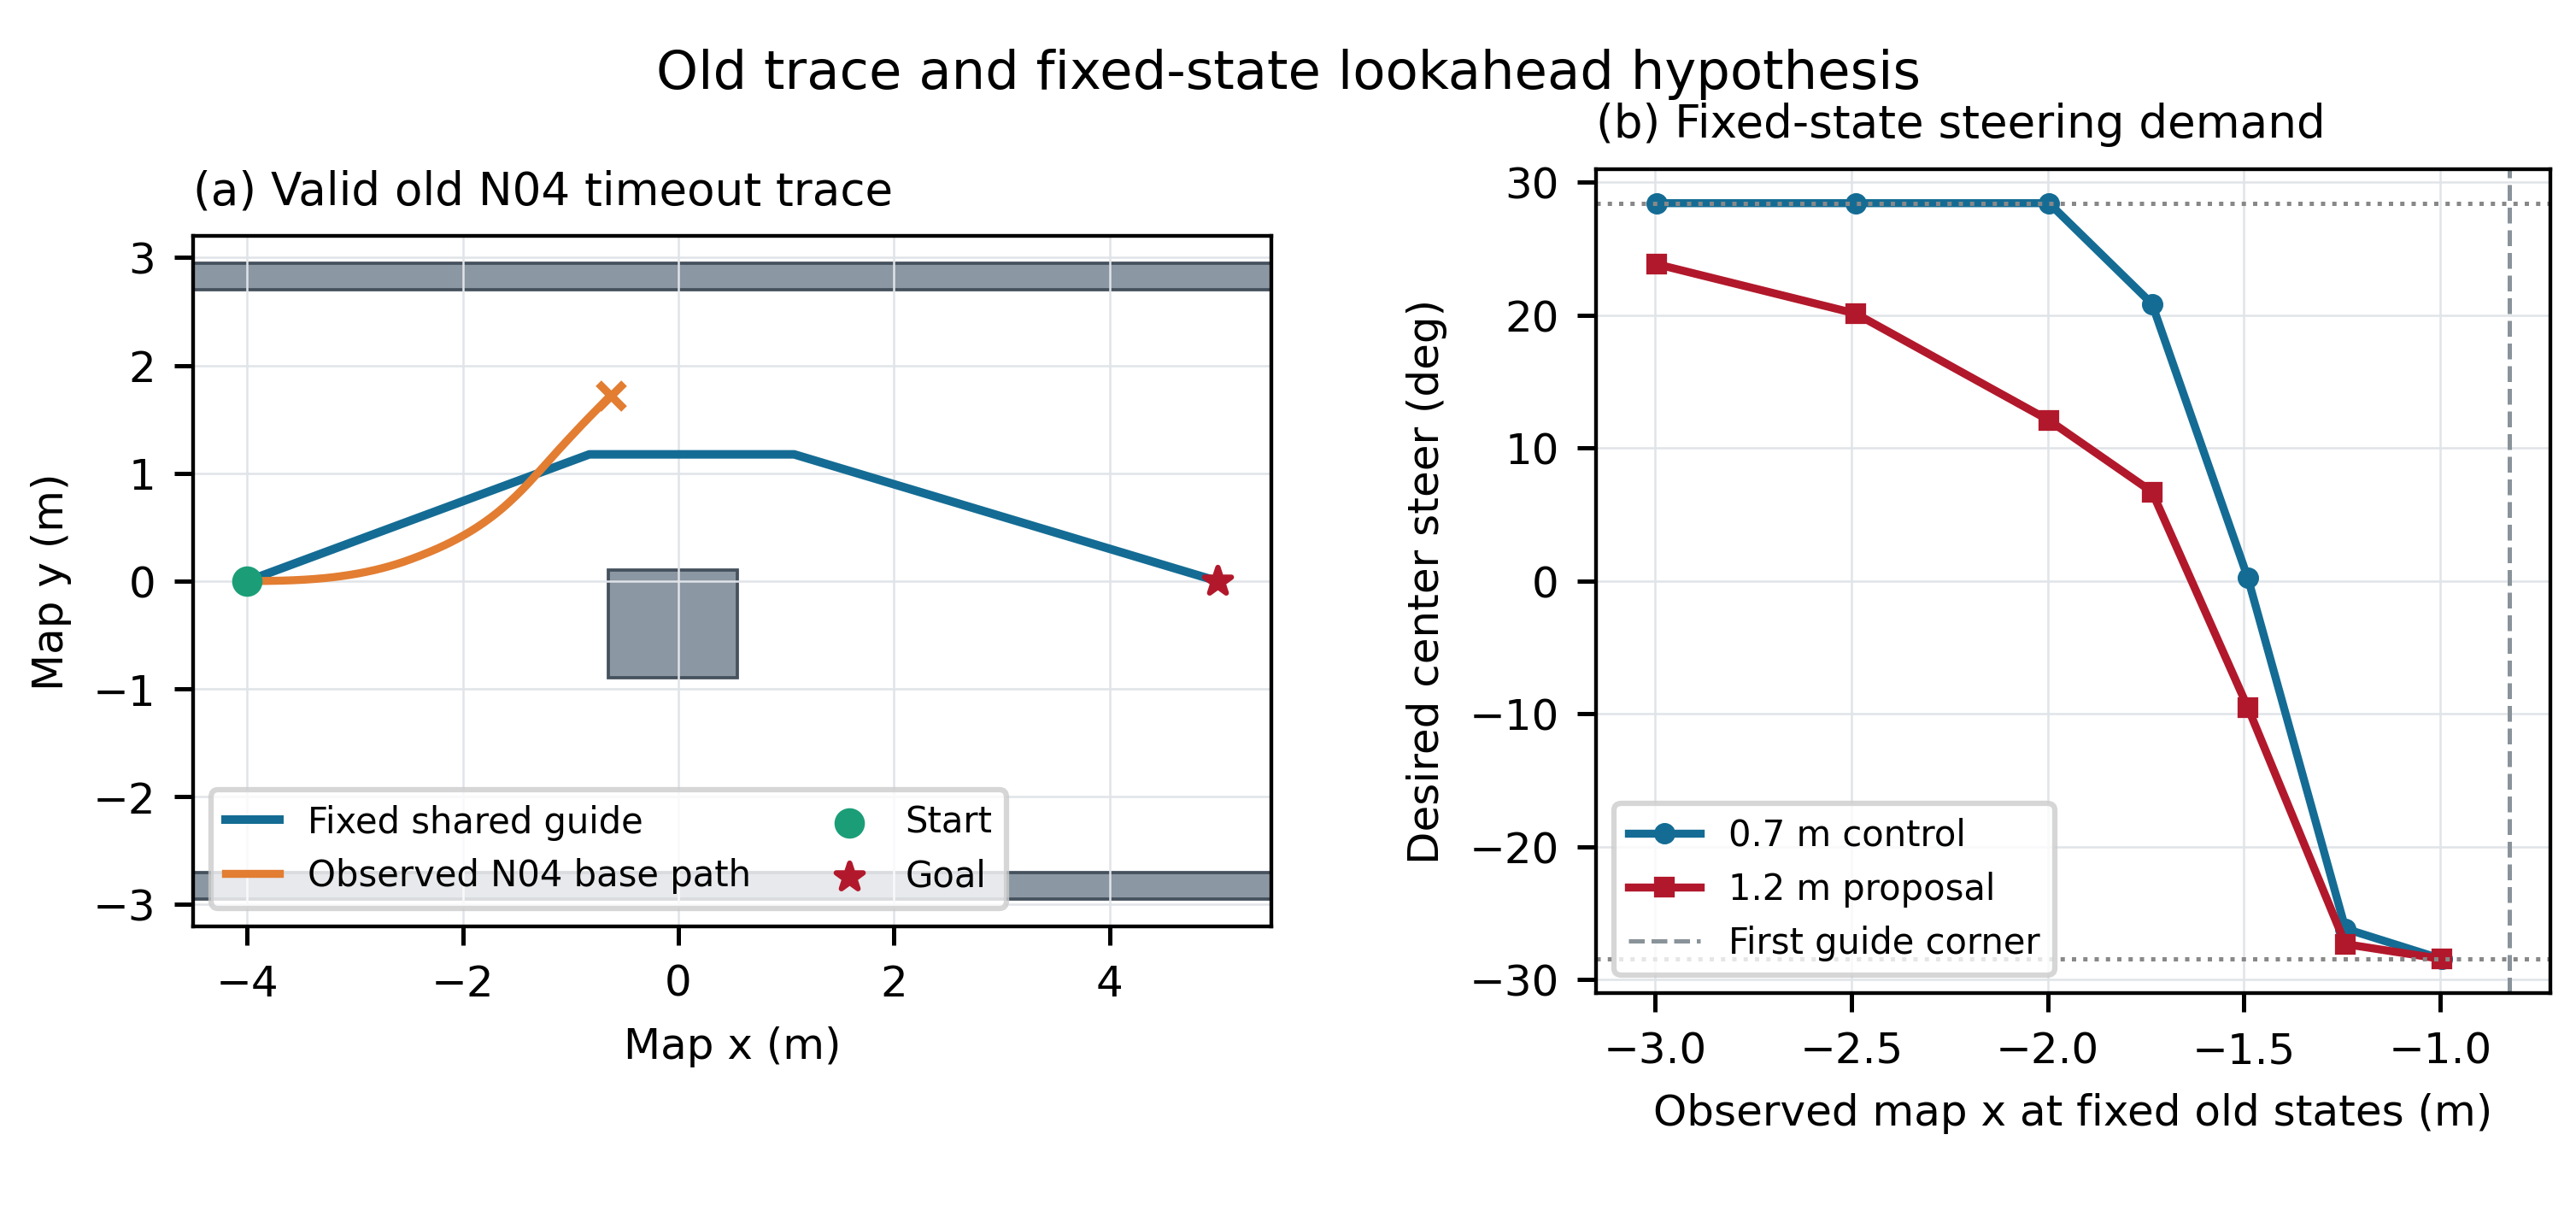
\includegraphics[width=\linewidth]{artifacts/astra_gazebo_20260926/paper_update/figures/NAV02_lookahead_fixed_state_diagnostic_r03/NAV02_lookahead_fixed_state_diagnostic.png}
  \caption{旧静态超时轨迹与固定状态前瞻假设。旧超时路径中前瞻距离变化如何影响相同状态下的期望转向}
  \label{fig:astra-nav02}
\end{figure}

\begin{figure}[tbp]
  \centering
  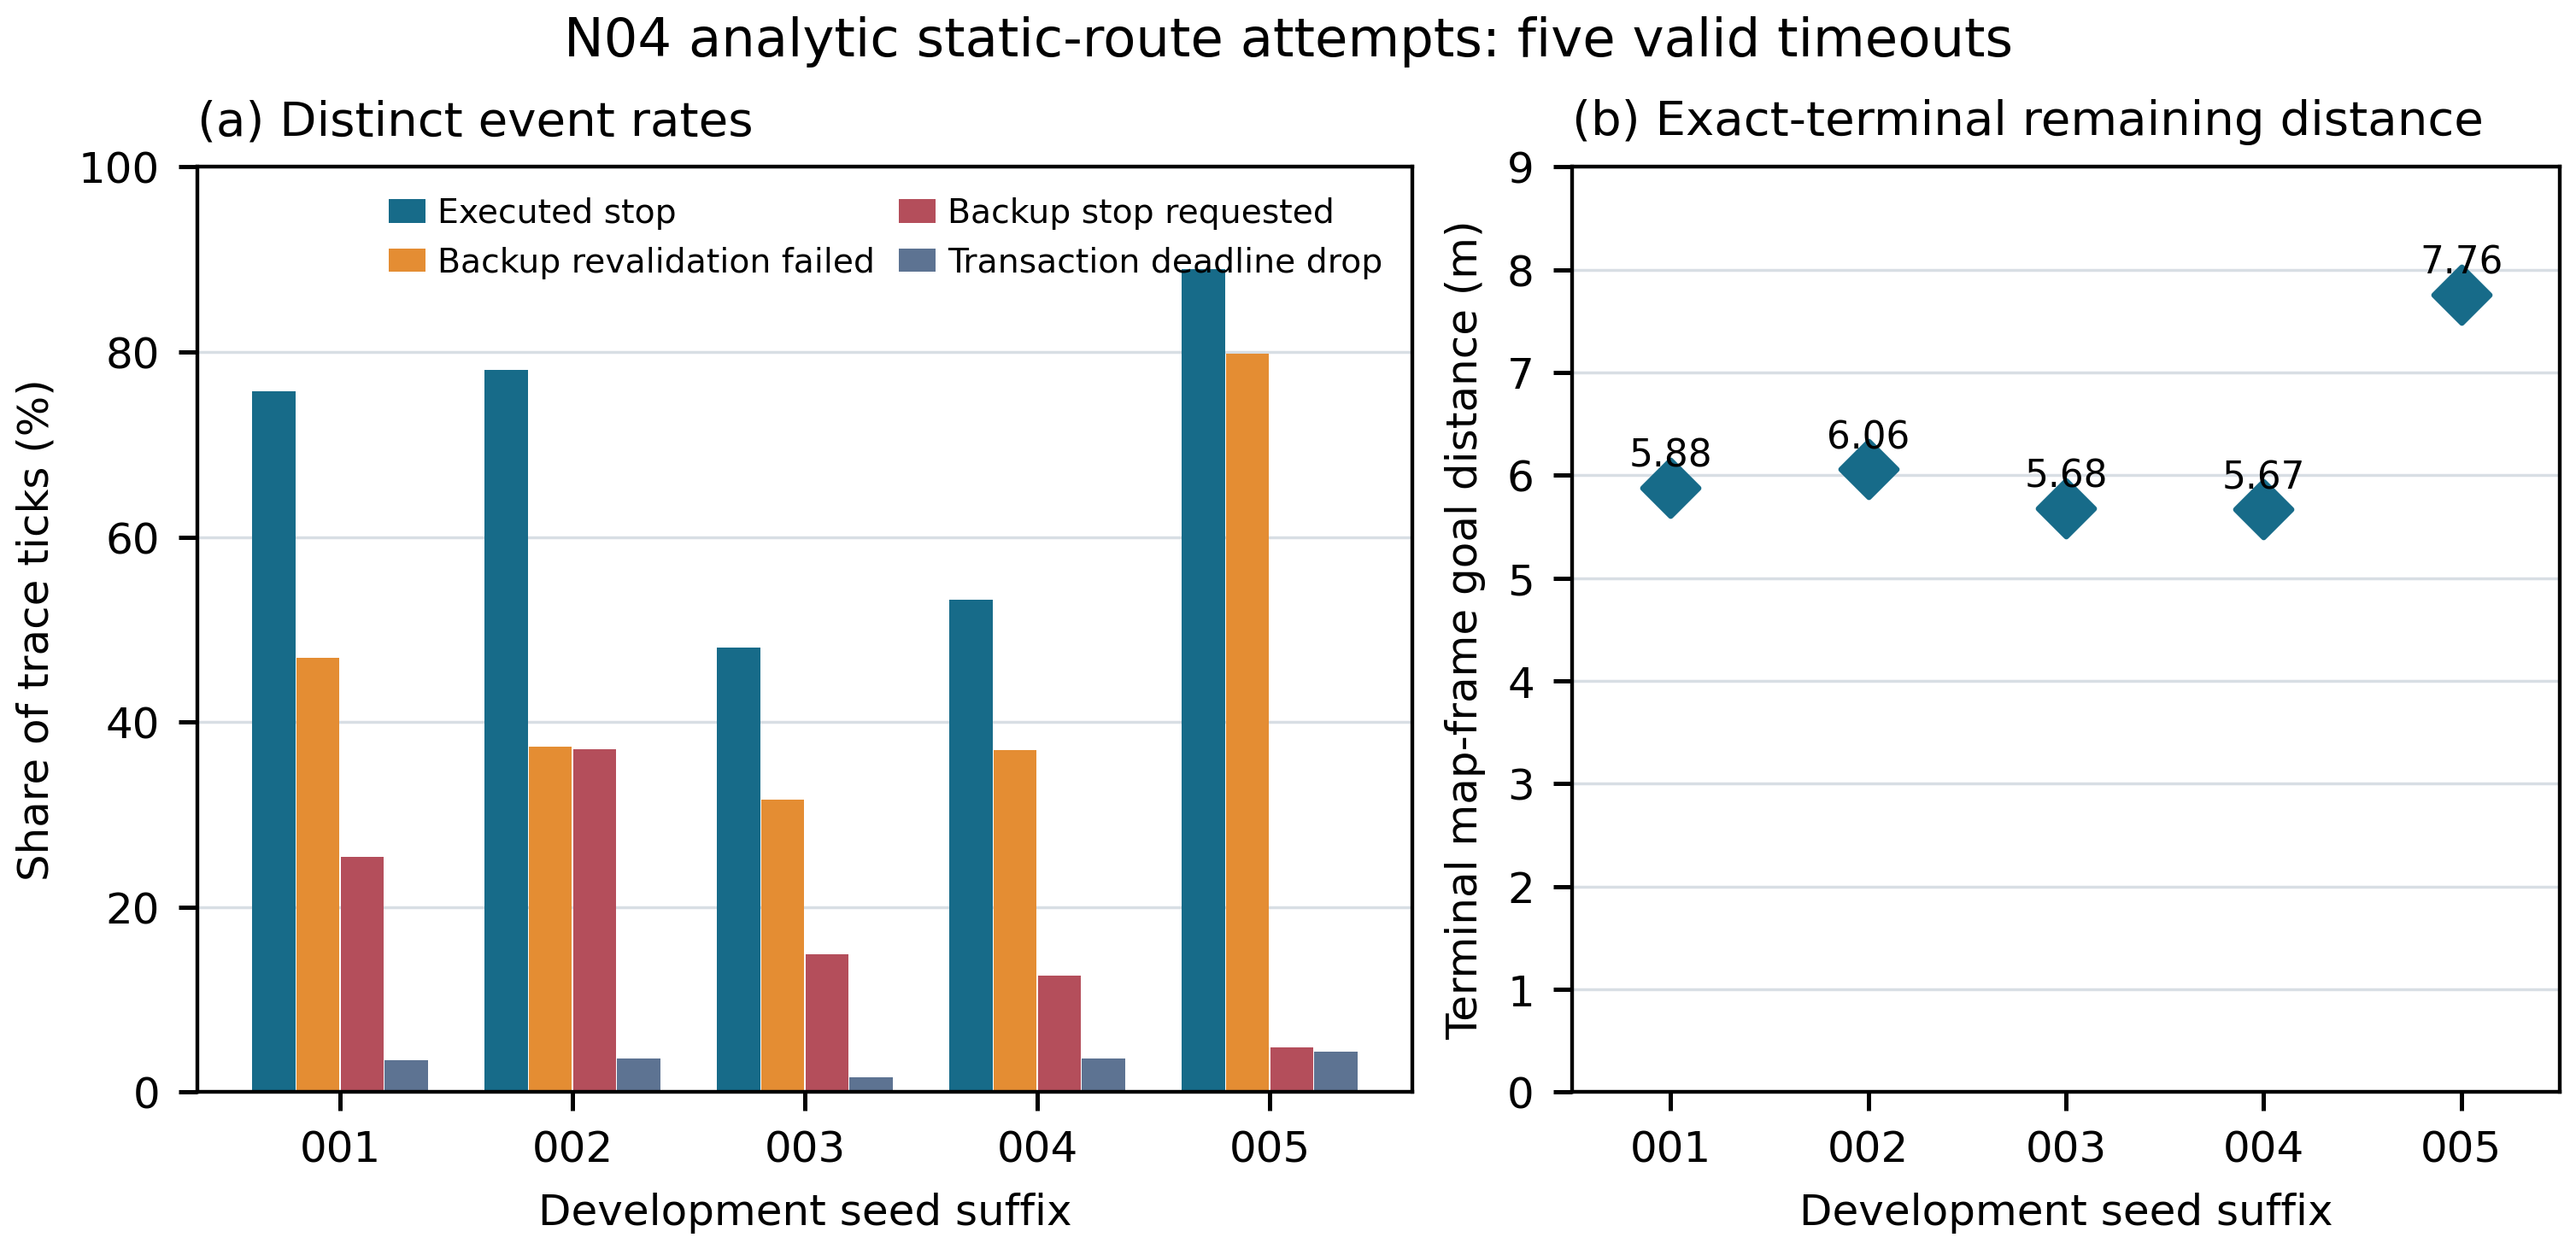
\includegraphics[width=\linewidth]{artifacts/astra_gazebo_20260926/paper_update/figures/NAV03_n04_five_attempts_r01/NAV03_n04_five_attempts.png}
  \caption{N04五次静态超时中的独立事件率与终态距离。五个旧开发回合的停止与退避相关事件是否一致以及终态距目标多远}
  \label{fig:astra-nav03}
\end{figure}

\begin{figure}[tbp]
  \centering
  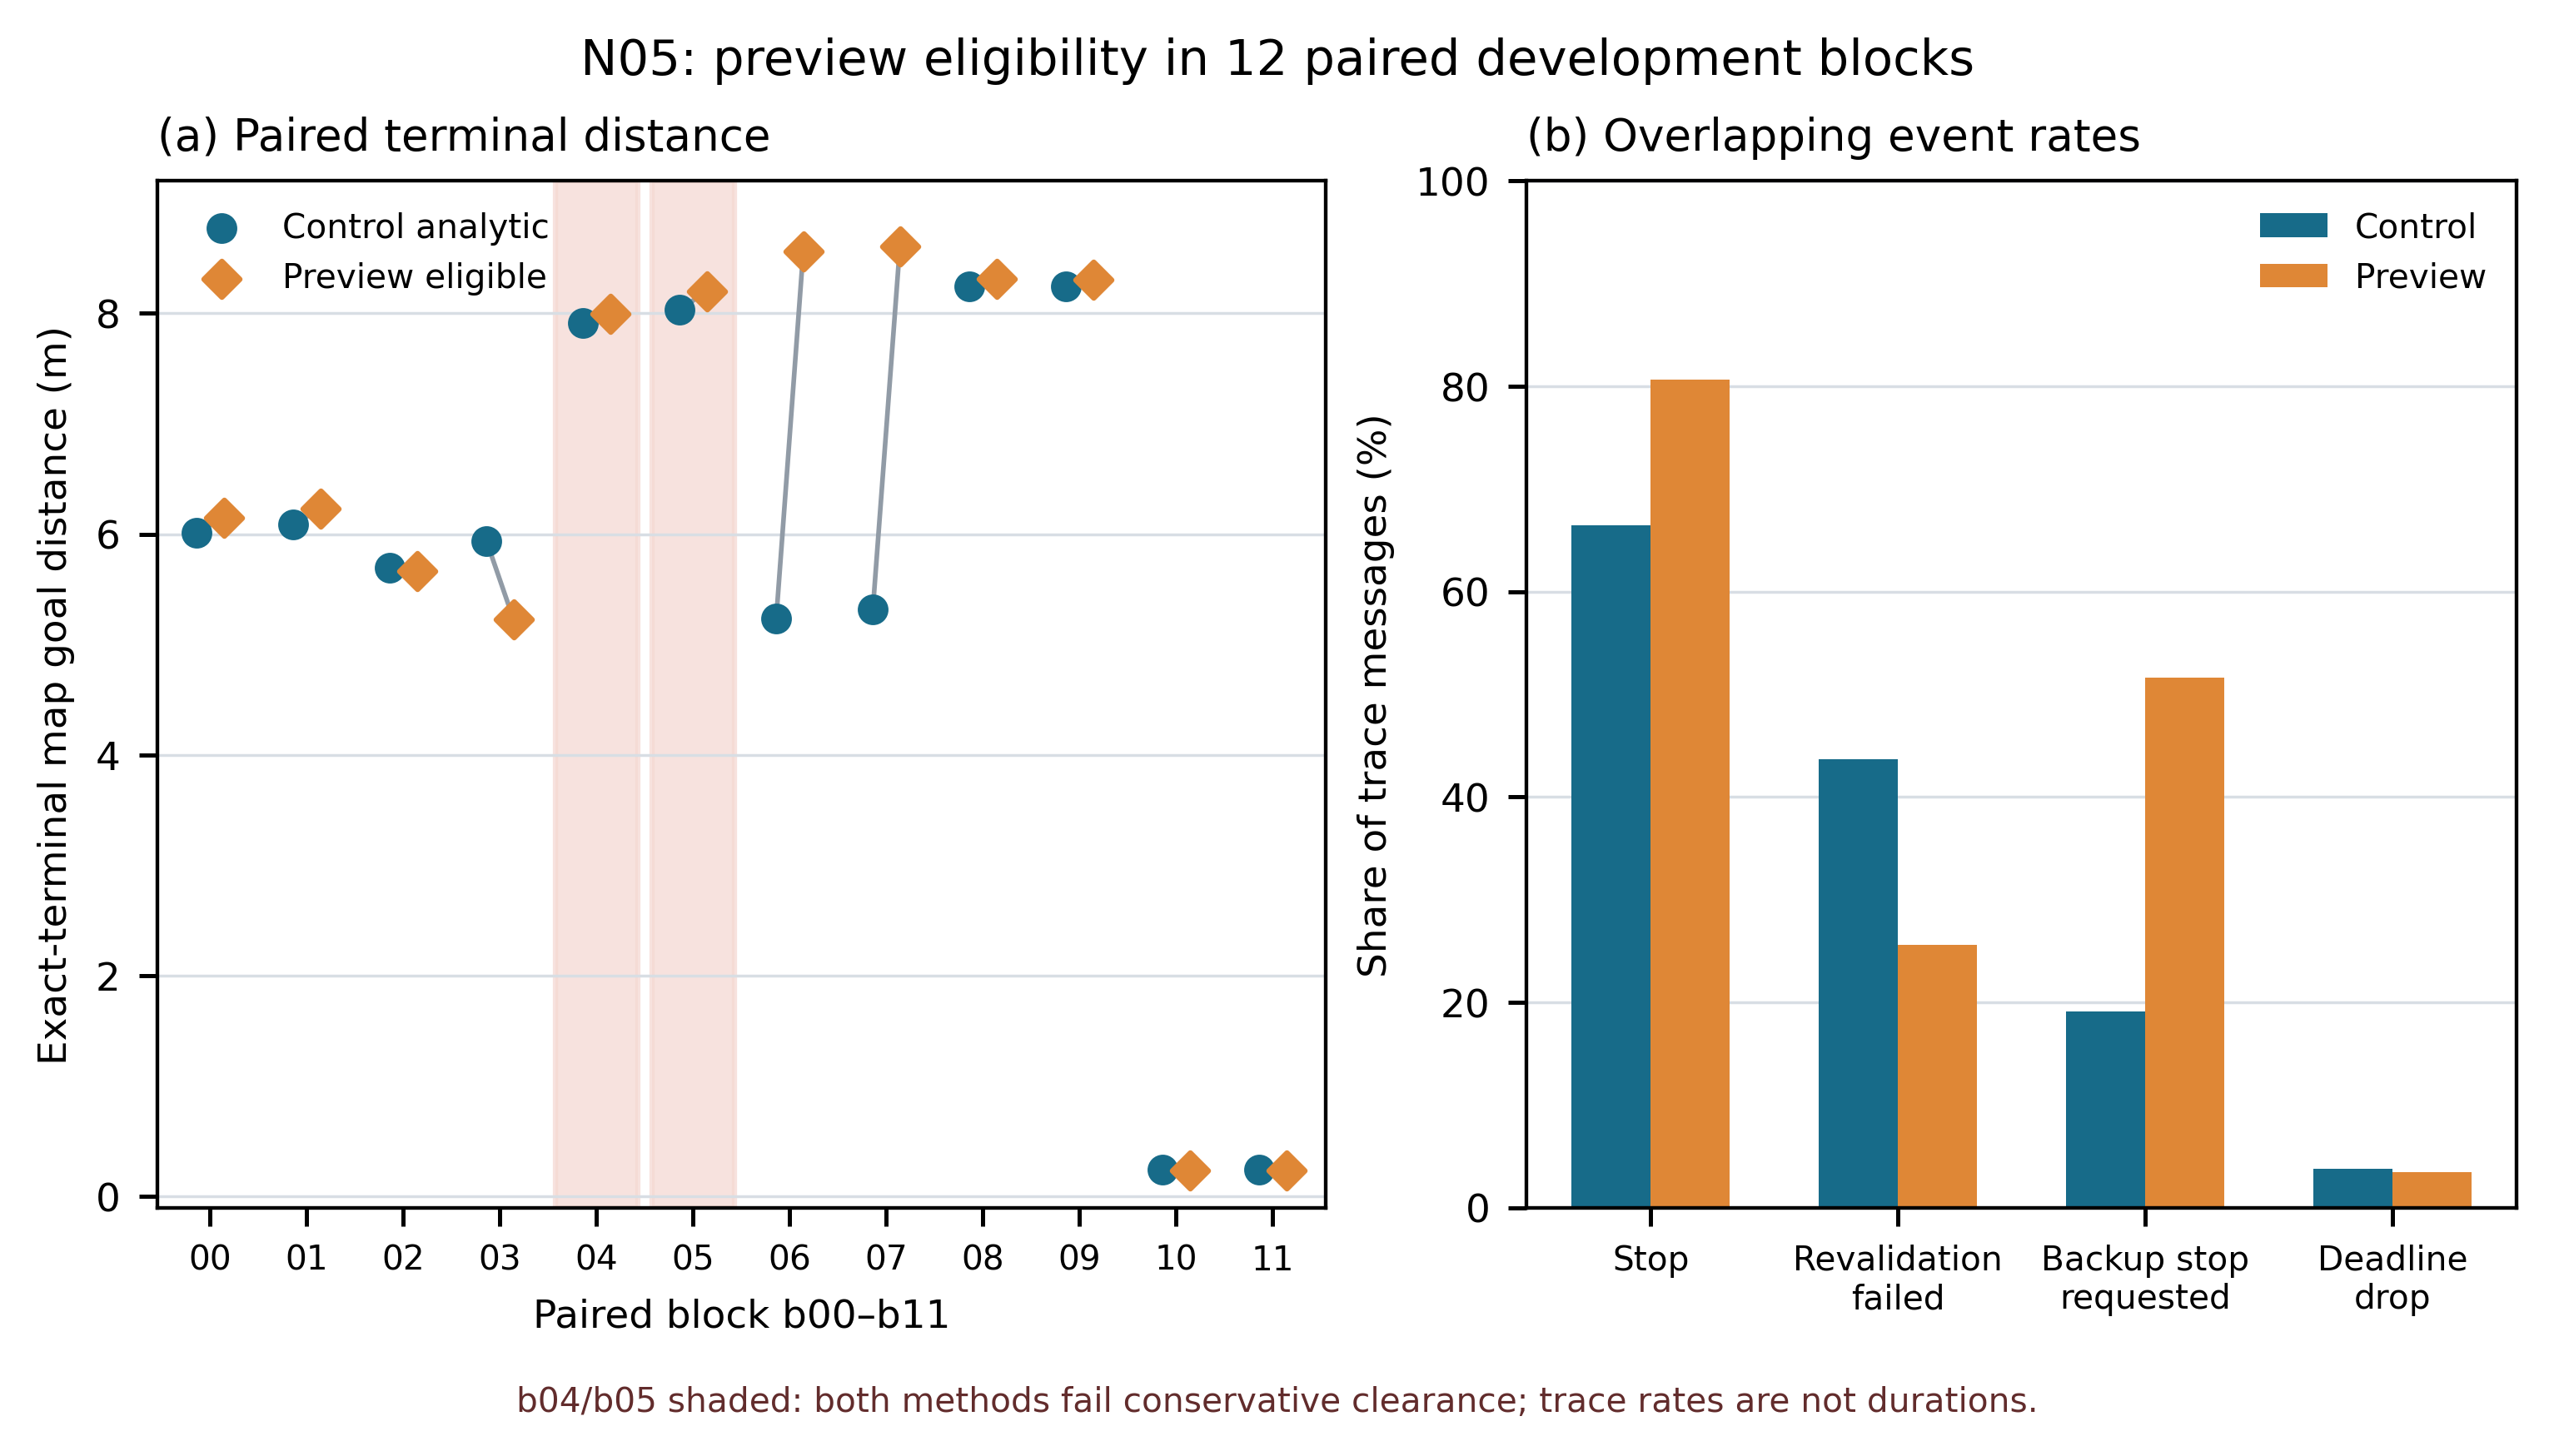
\includegraphics[width=\linewidth]{artifacts/astra_gazebo_20260926/paper_update/figures/NAV04_n05_paired_diagnostic_r02/NAV04_n05_paired_diagnostic.png}
  \caption{N05配对终态距离与重叠事件率。预览可选性约束改变动作后是否改善旧开发几何的结果}
  \label{fig:astra-nav04}
\end{figure}

\begin{figure}[tbp]
  \centering
  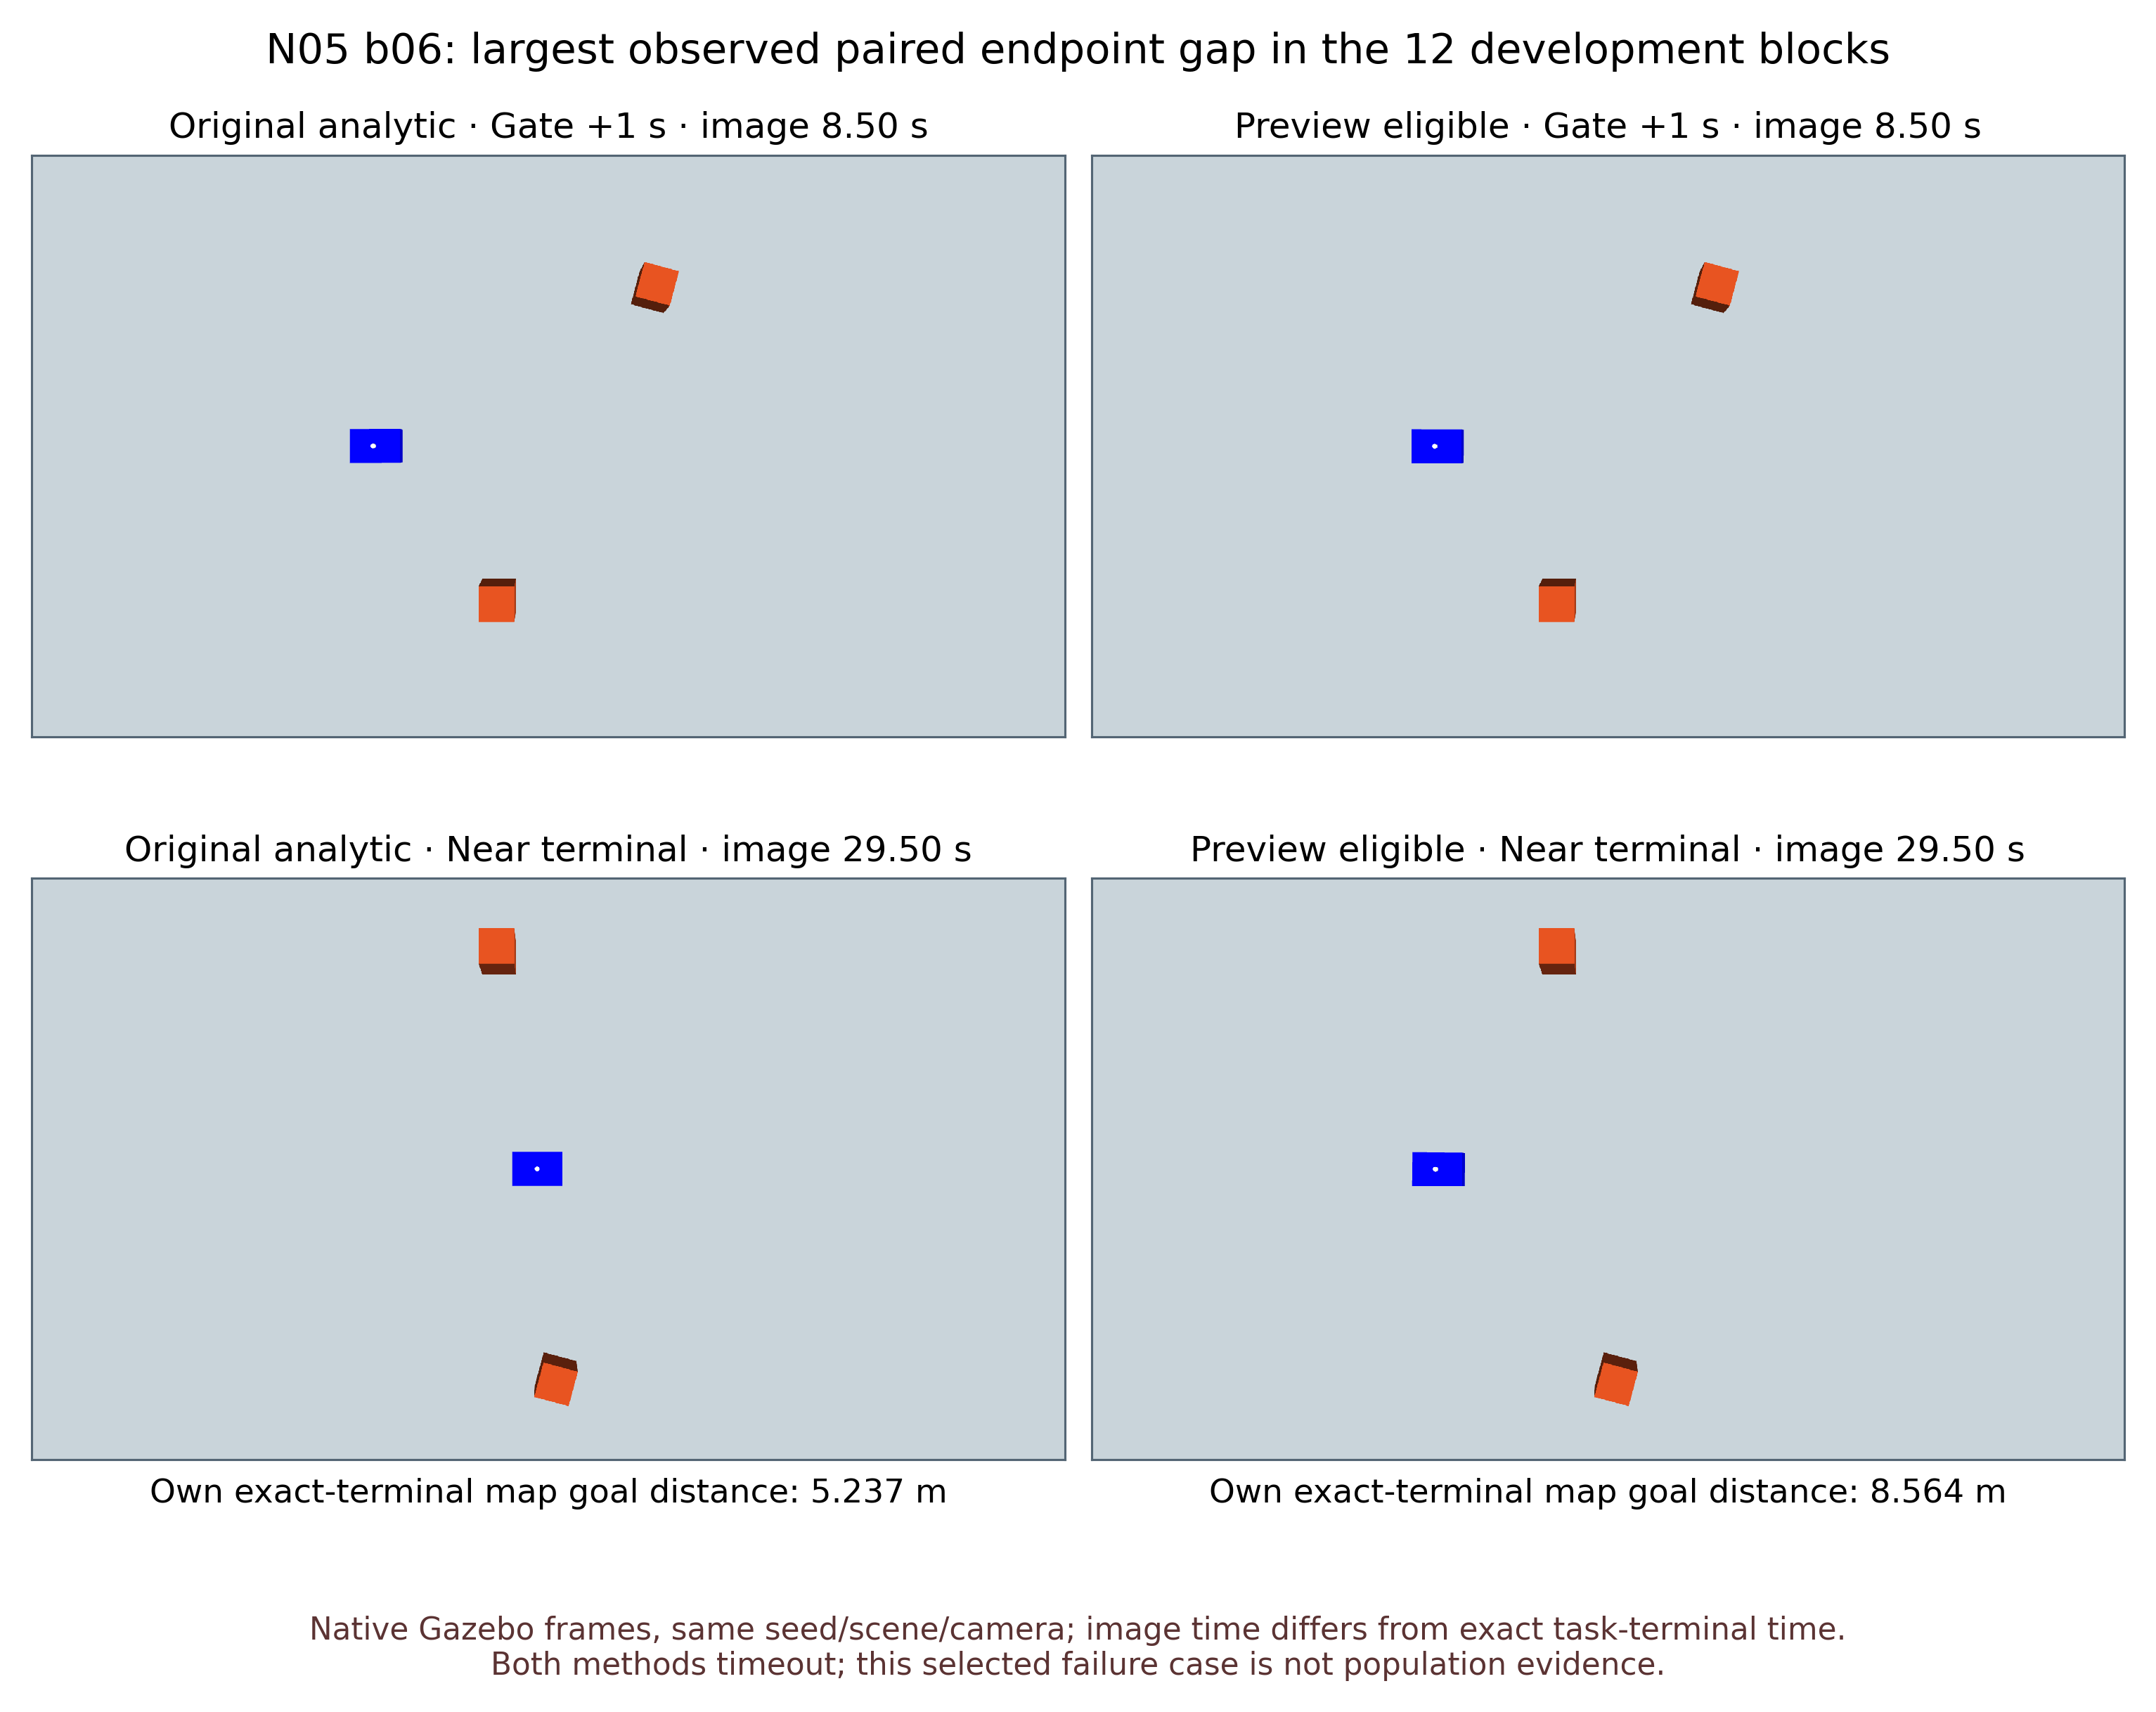
\includegraphics[width=\linewidth]{artifacts/astra_gazebo_20260926/paper_update/figures/NAV05_n05_native_pair_r02/NAV05_n05_native_pair.png}
  \caption{N05最大终态差配对的原生仿真截图。同一新seed/场景下两方法从相同早期画面到终态如何分化}
  \label{fig:astra-nav05}
\end{figure}

\begin{figure}[tbp]
  \centering
  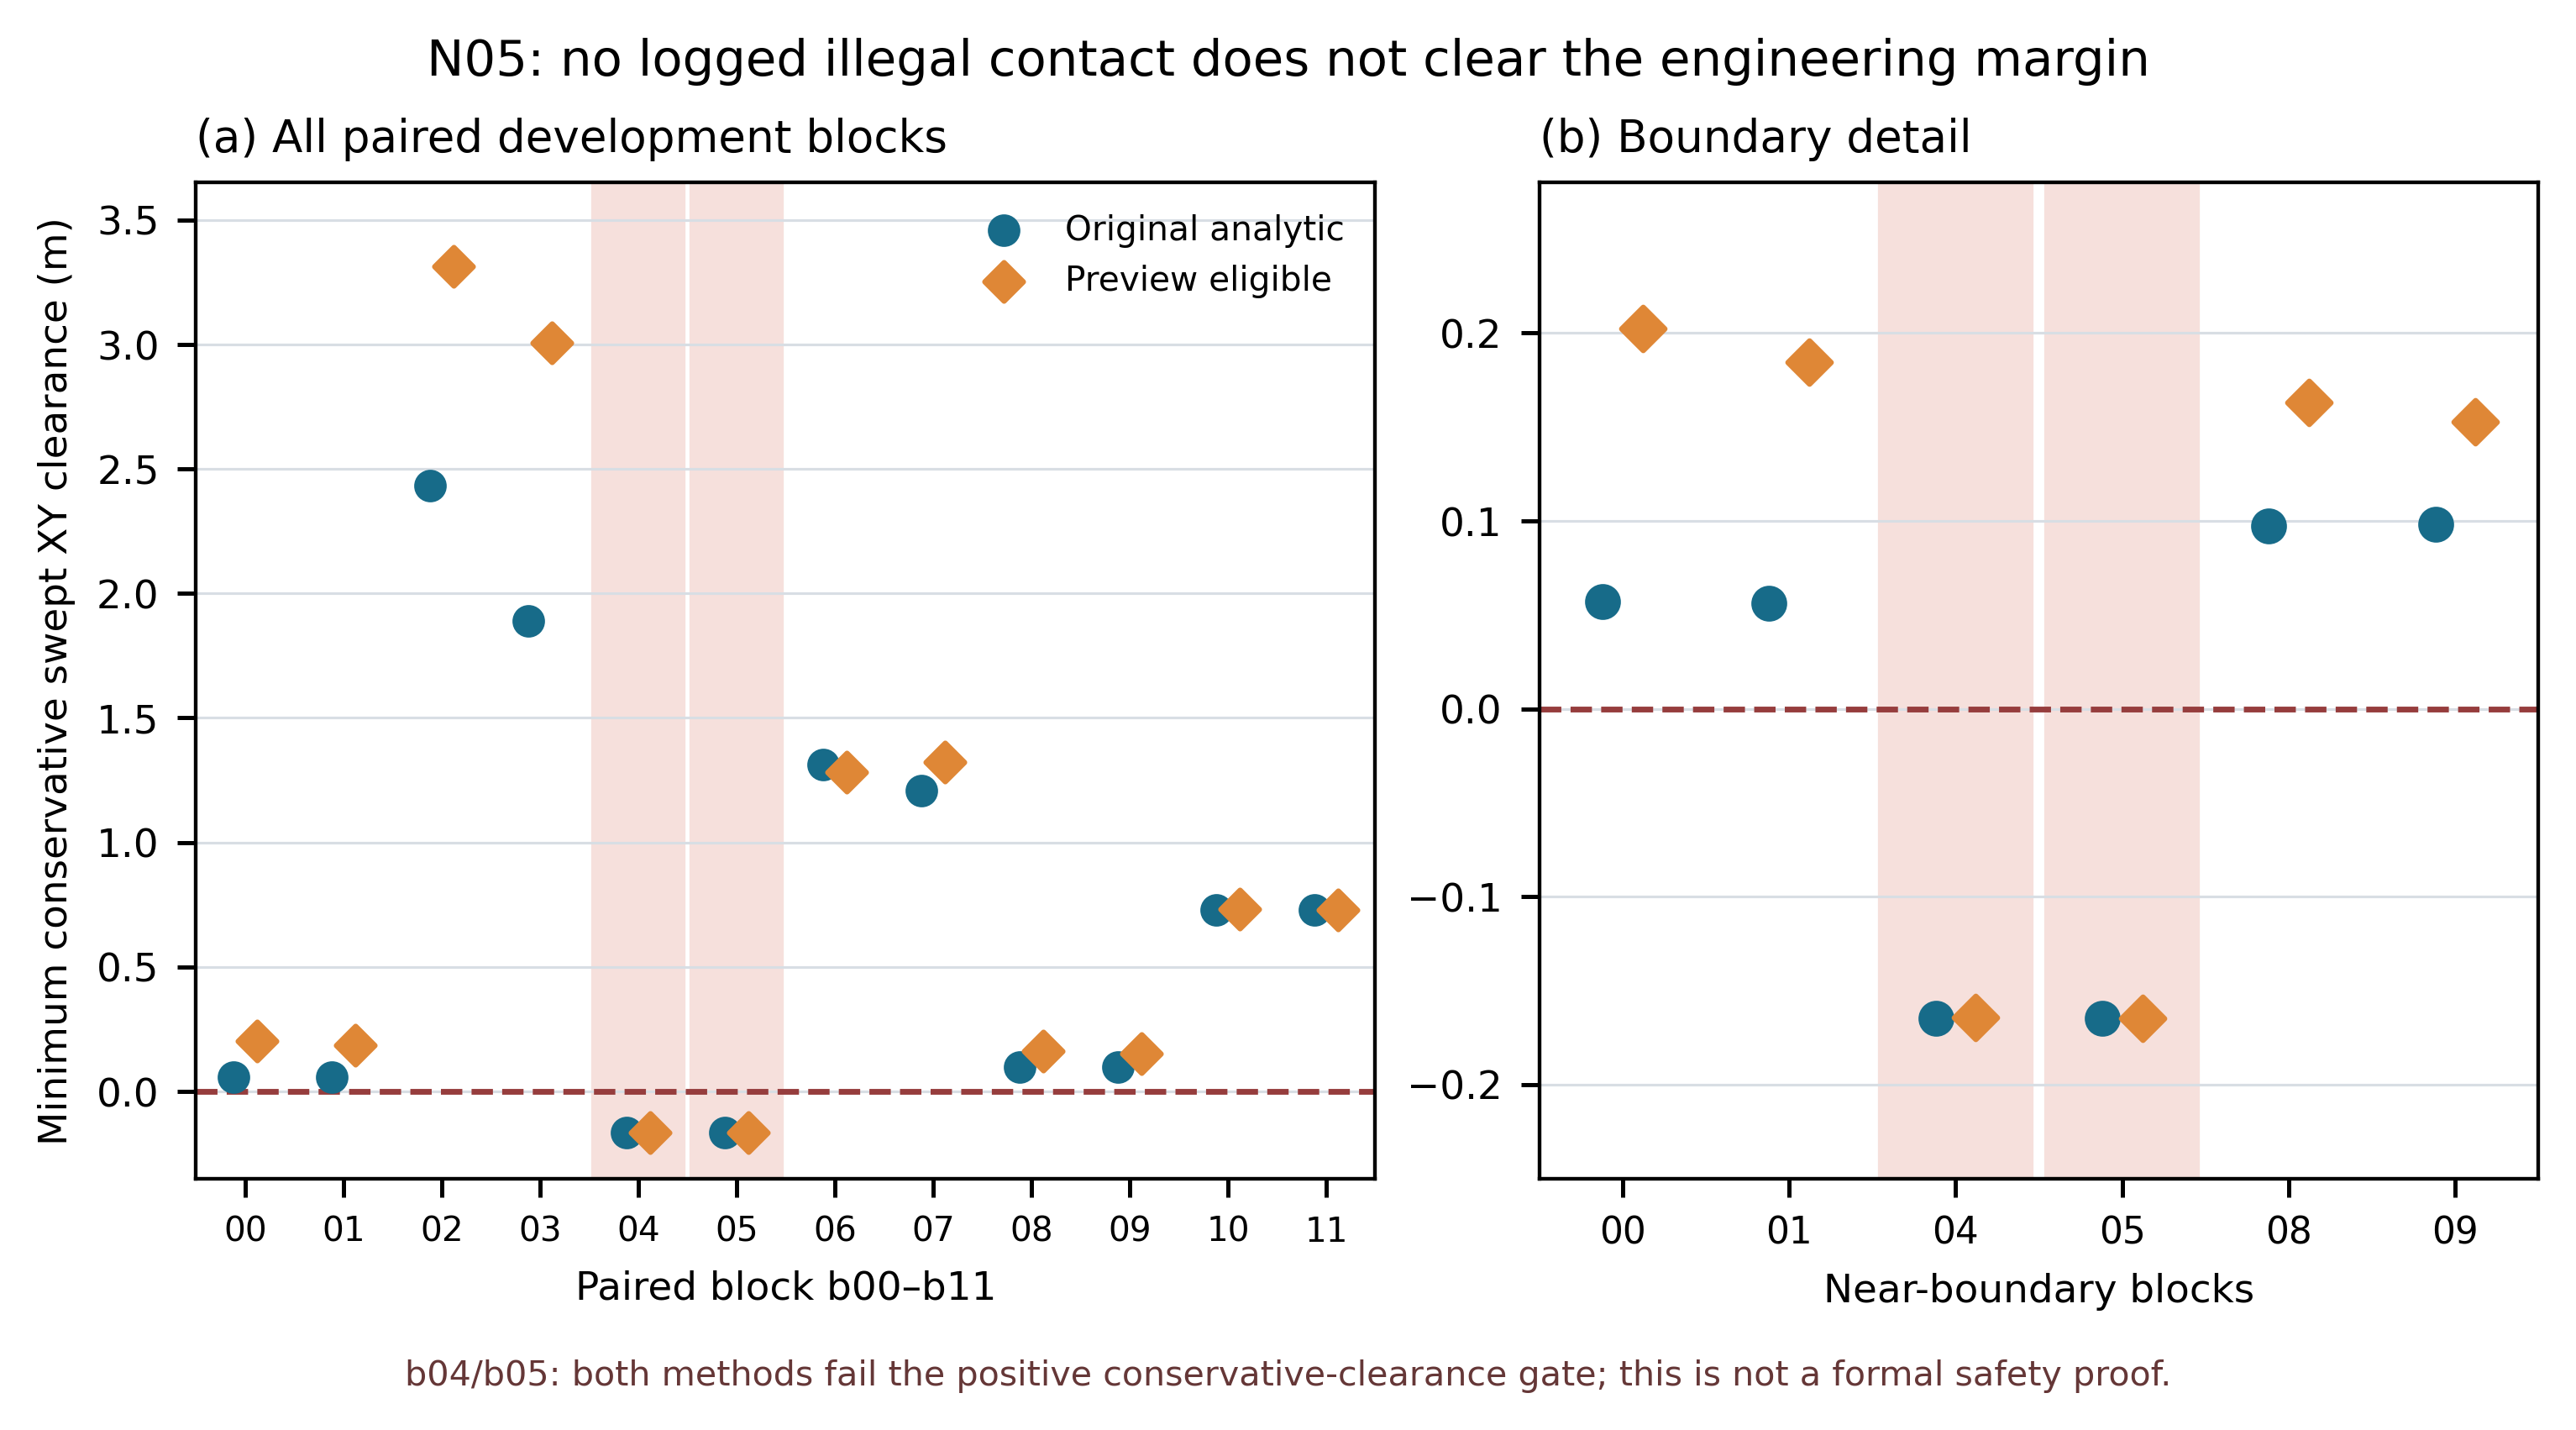
\includegraphics[width=\linewidth]{artifacts/astra_gazebo_20260926/paper_update/figures/NAV06_n05_clearance_gate_r01/NAV06_n05_clearance_gate.png}
  \caption{N05保守扫掠净距安全门。零违法接触日志能否排除保守工程净距失败}
  \label{fig:astra-nav06}
\end{figure}

\begin{figure}[tbp]
  \centering
  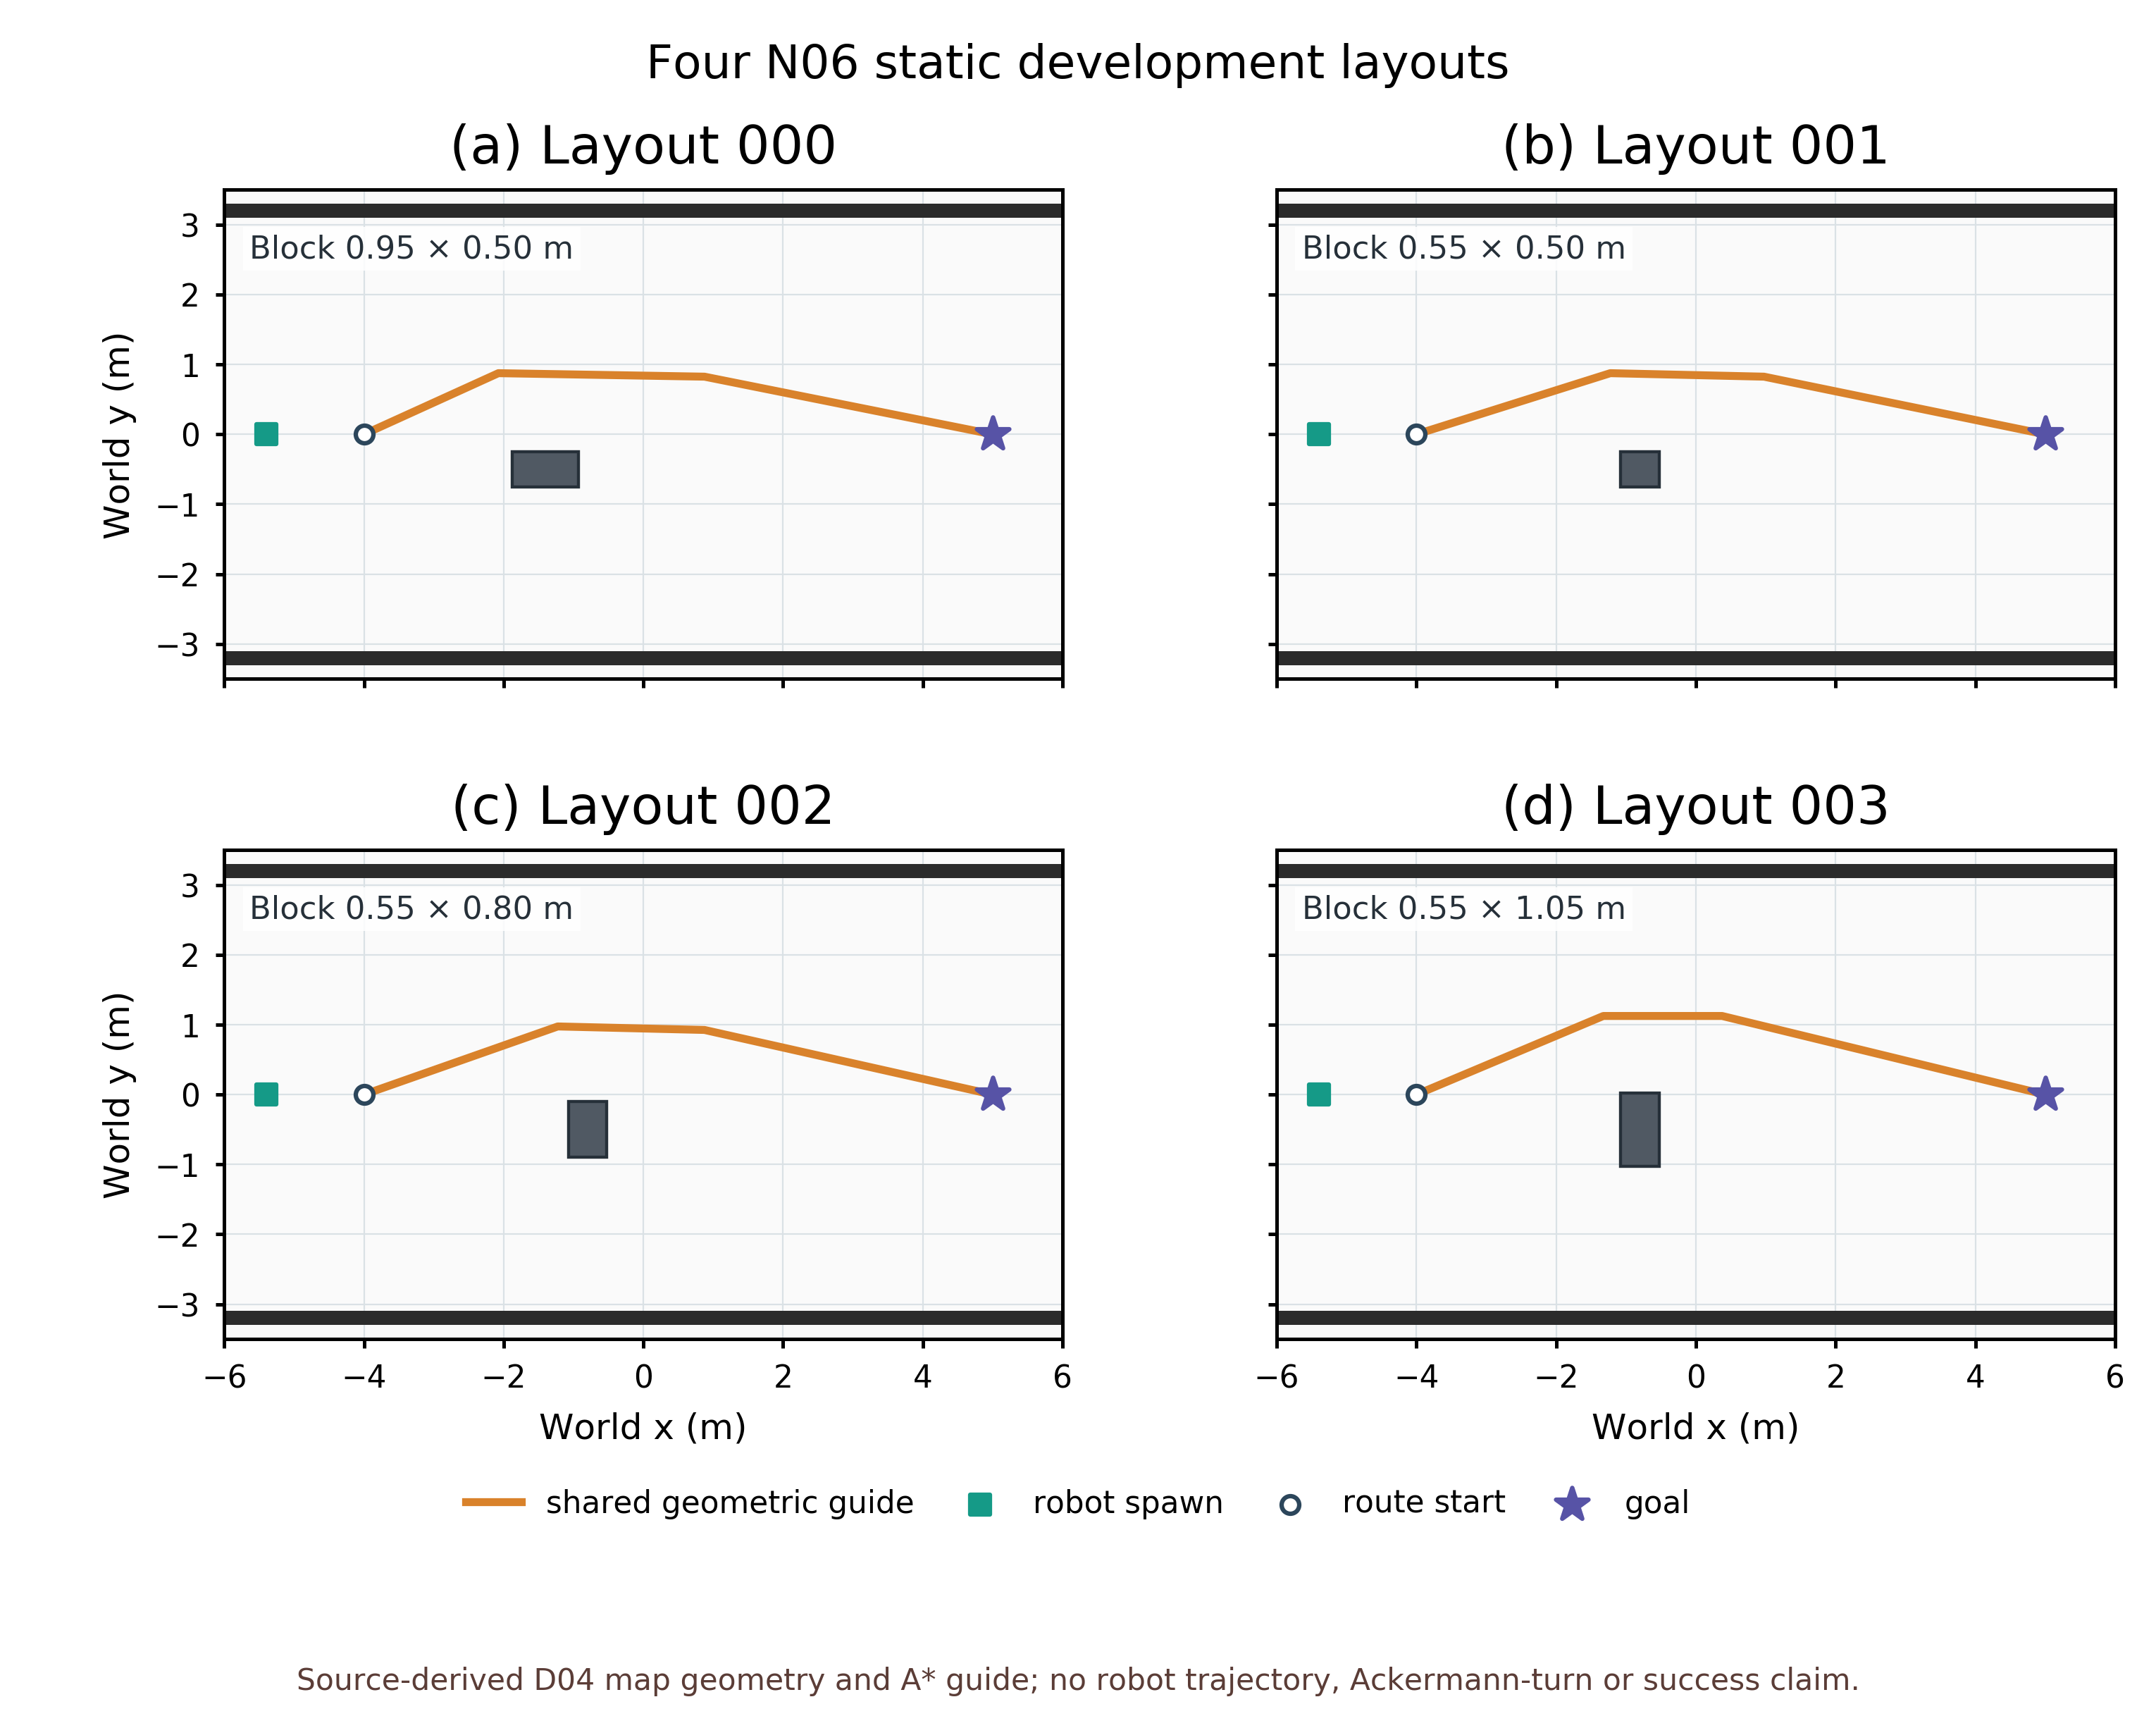
\includegraphics[width=\linewidth]{artifacts/astra_gazebo_20260926/paper_update/figures/NAV07_d04_static_layouts_r03/NAV07_d04_static_layouts.png}
  \caption{N06四个新静态开发布局与共用几何引导线。单因素静态先导试验使用了哪些独立新场景}
  \label{fig:astra-nav07}
\end{figure}

\begin{figure}[tbp]
  \centering
  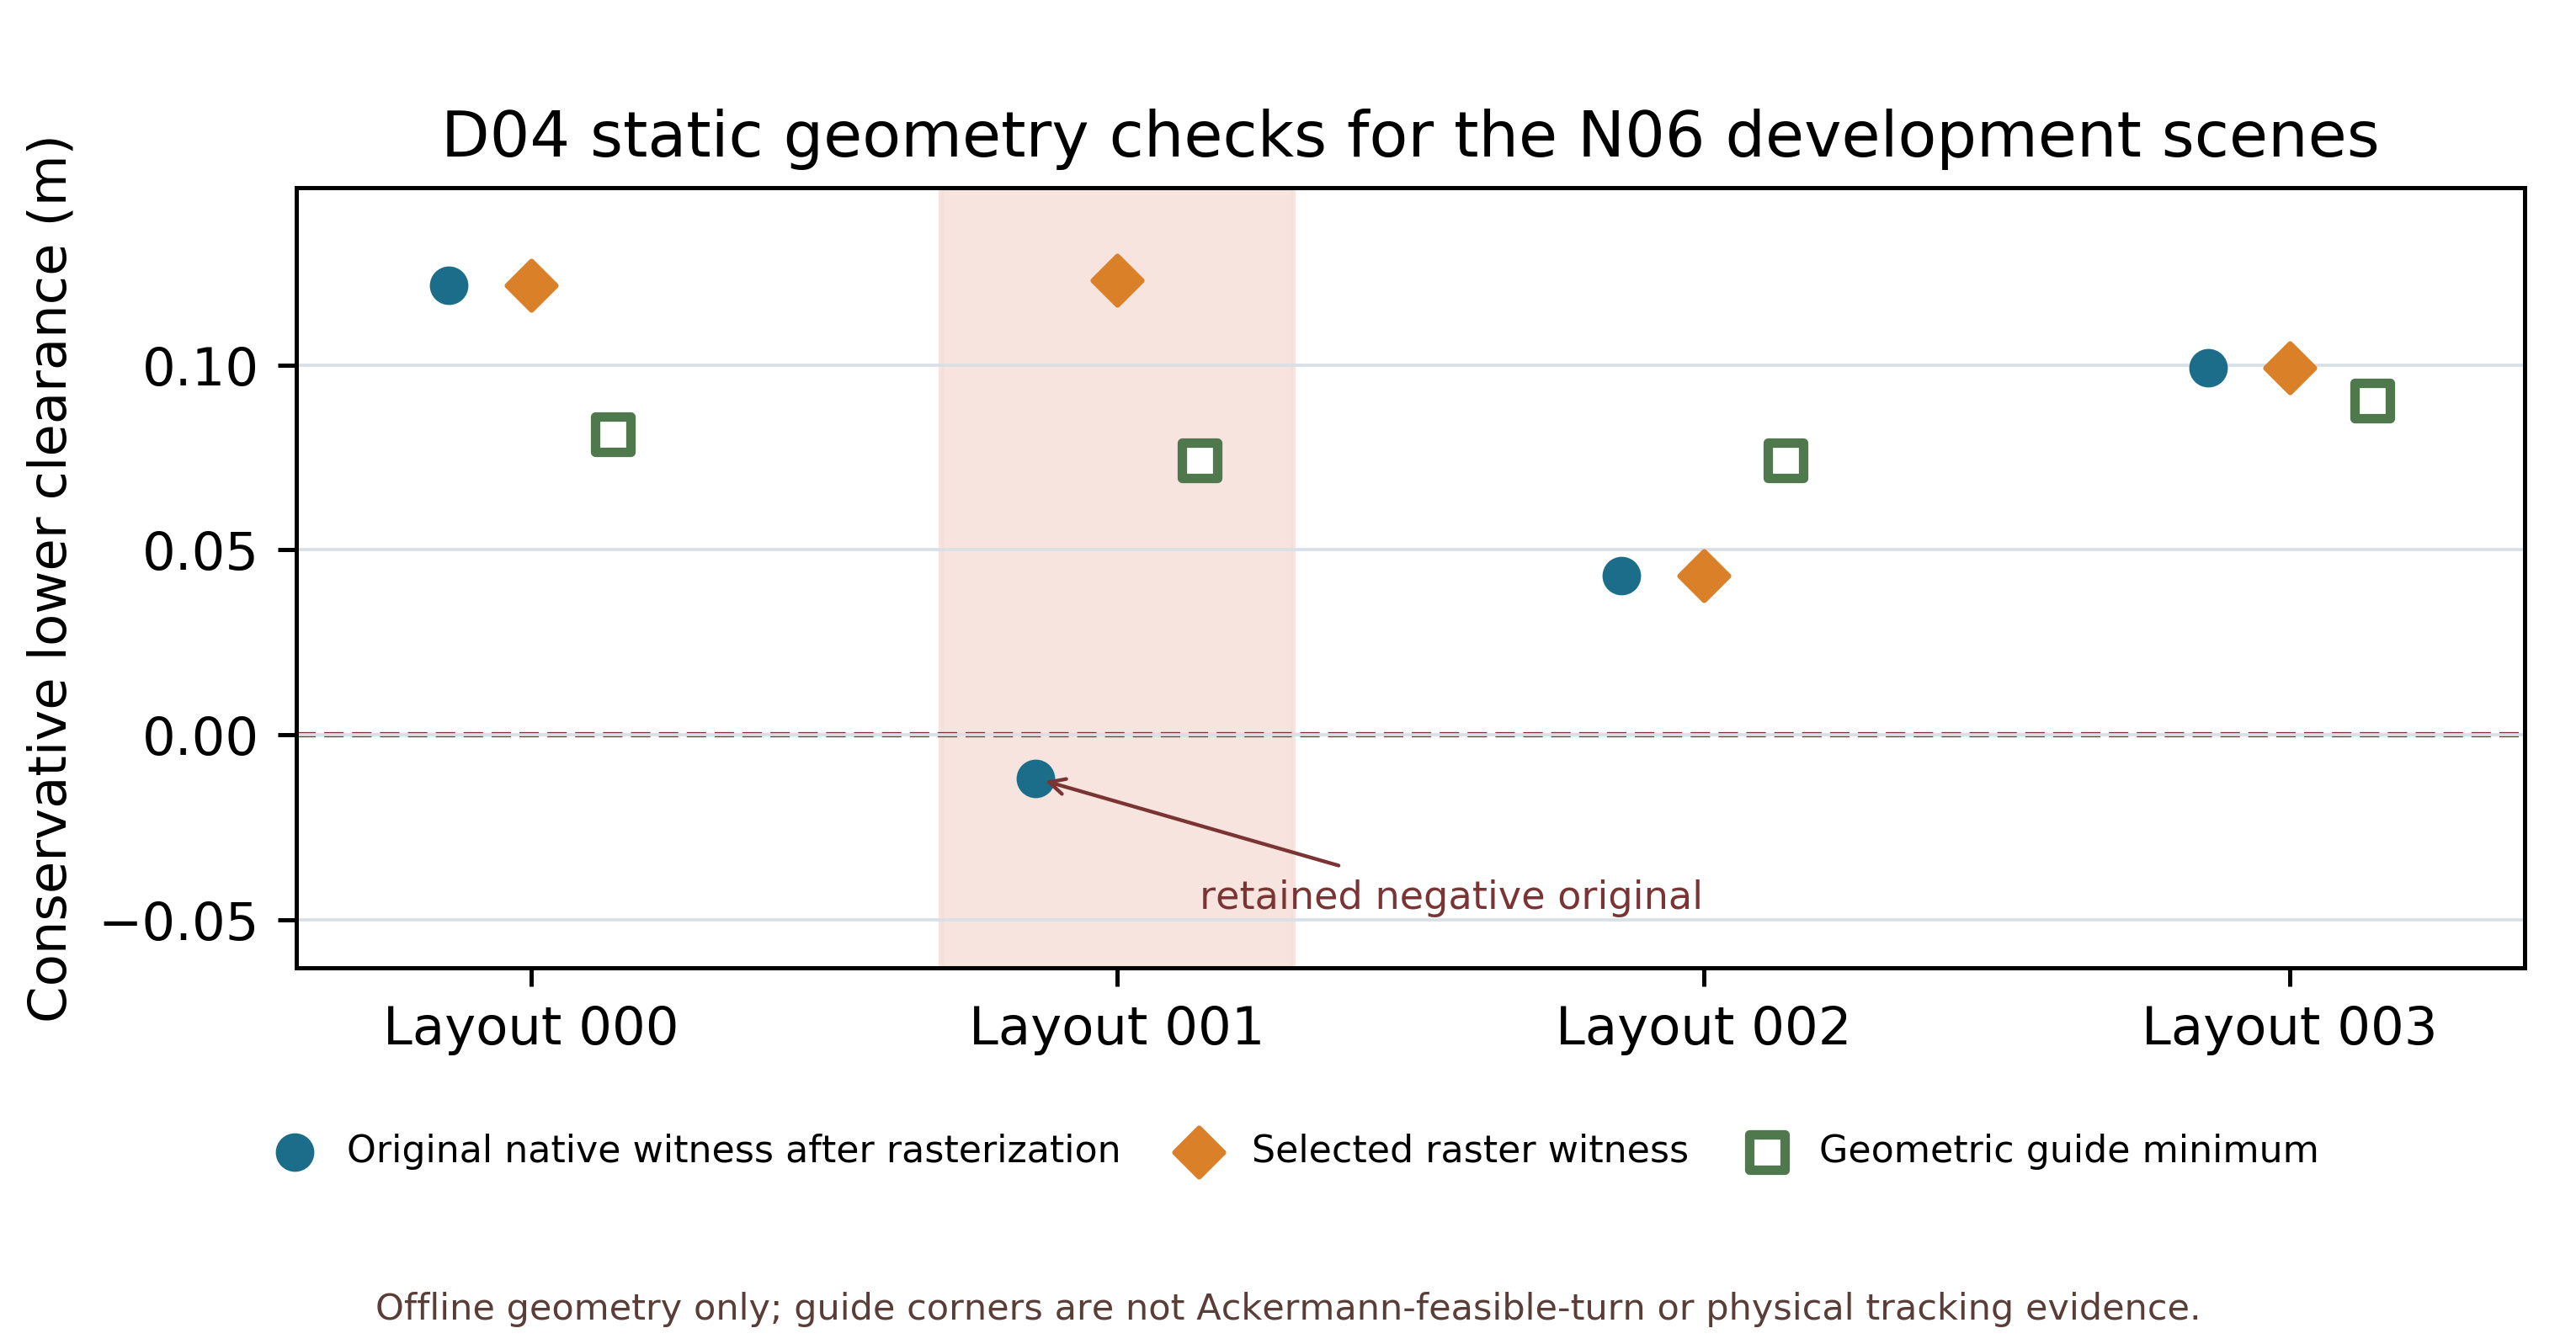
\includegraphics[width=\linewidth]{artifacts/astra_gazebo_20260926/paper_update/figures/NAV08_d04_static_geometry_margins_r02/NAV08_d04_static_geometry_margins.png}
  \caption{D04四个新静态场景的离线保守几何净距。被替代的负值原见证路径与选定路径是否如实保留}
  \label{fig:astra-nav08}
\end{figure}
